Im folgenden Teil des Fachberichtes wird der Aufbau der Software beschrieben. Es folgt zu Beginn eine Gesamtübersicht und ein Kommentar zur Auswahl der verwendeten Programmiersprachen und Schnittstellen. Danach werden die einzelnen Teilsysteme beschrieben.

\textbf{Übersicht}\\
Die Software ermöglicht die Bedienung des Ultraschall Phased Array Systems über eine Web\-applikation. Anhand der Benutzereingaben werden auf dem Arduino automatisch Messungen durchgeführt und die Resultate im User-Interface dargestellt.

Auf dem Arduino DUE wird eine in C programmierte Statemachine ausgeführt, diese übernimmt die Steuerung der Hardware. Abseits vom Arduino DUE ist die Software als Webapplikation realisiert, dabei wird grob zwischen host- und clientseitiger Software unterschieden.
Der hostseitige Code ist in der Programmiersprache Python realisiert und wird von einem pythonfähigen Desktop-Betriebssystem ausgeführt.
Der clientseitige Code wird, falls gewünscht, auf einem anderen Computer/Betriebssystem ausgeführt. Das User-Interface wird über einen Webbrowser aufgerufen und ist in den Programmiersprachen HTML, CSS und Java\-script umgesetzt.
Näheres zur Installation und Kompatibilität ist in dem Kapitel \ref{sec:entwicklungsumgebung} zu finden.

Die Dokumentation der Software wird aufgeteilt in drei verschiedene Teilsysteme. Abbildung \ref{fig:image_software_schema}  enthält eine Übersicht über die gesamte Software.

%%%%%%%%%%%%%%%%%%%%%%%%%%%%%%%%%%%%%%%%%%%%%%%%%%%%%%%%%%%%%%%%%%%%%%%%%%%%%%%%
% pictures
\begin{figure}[htb]
\begin{center}
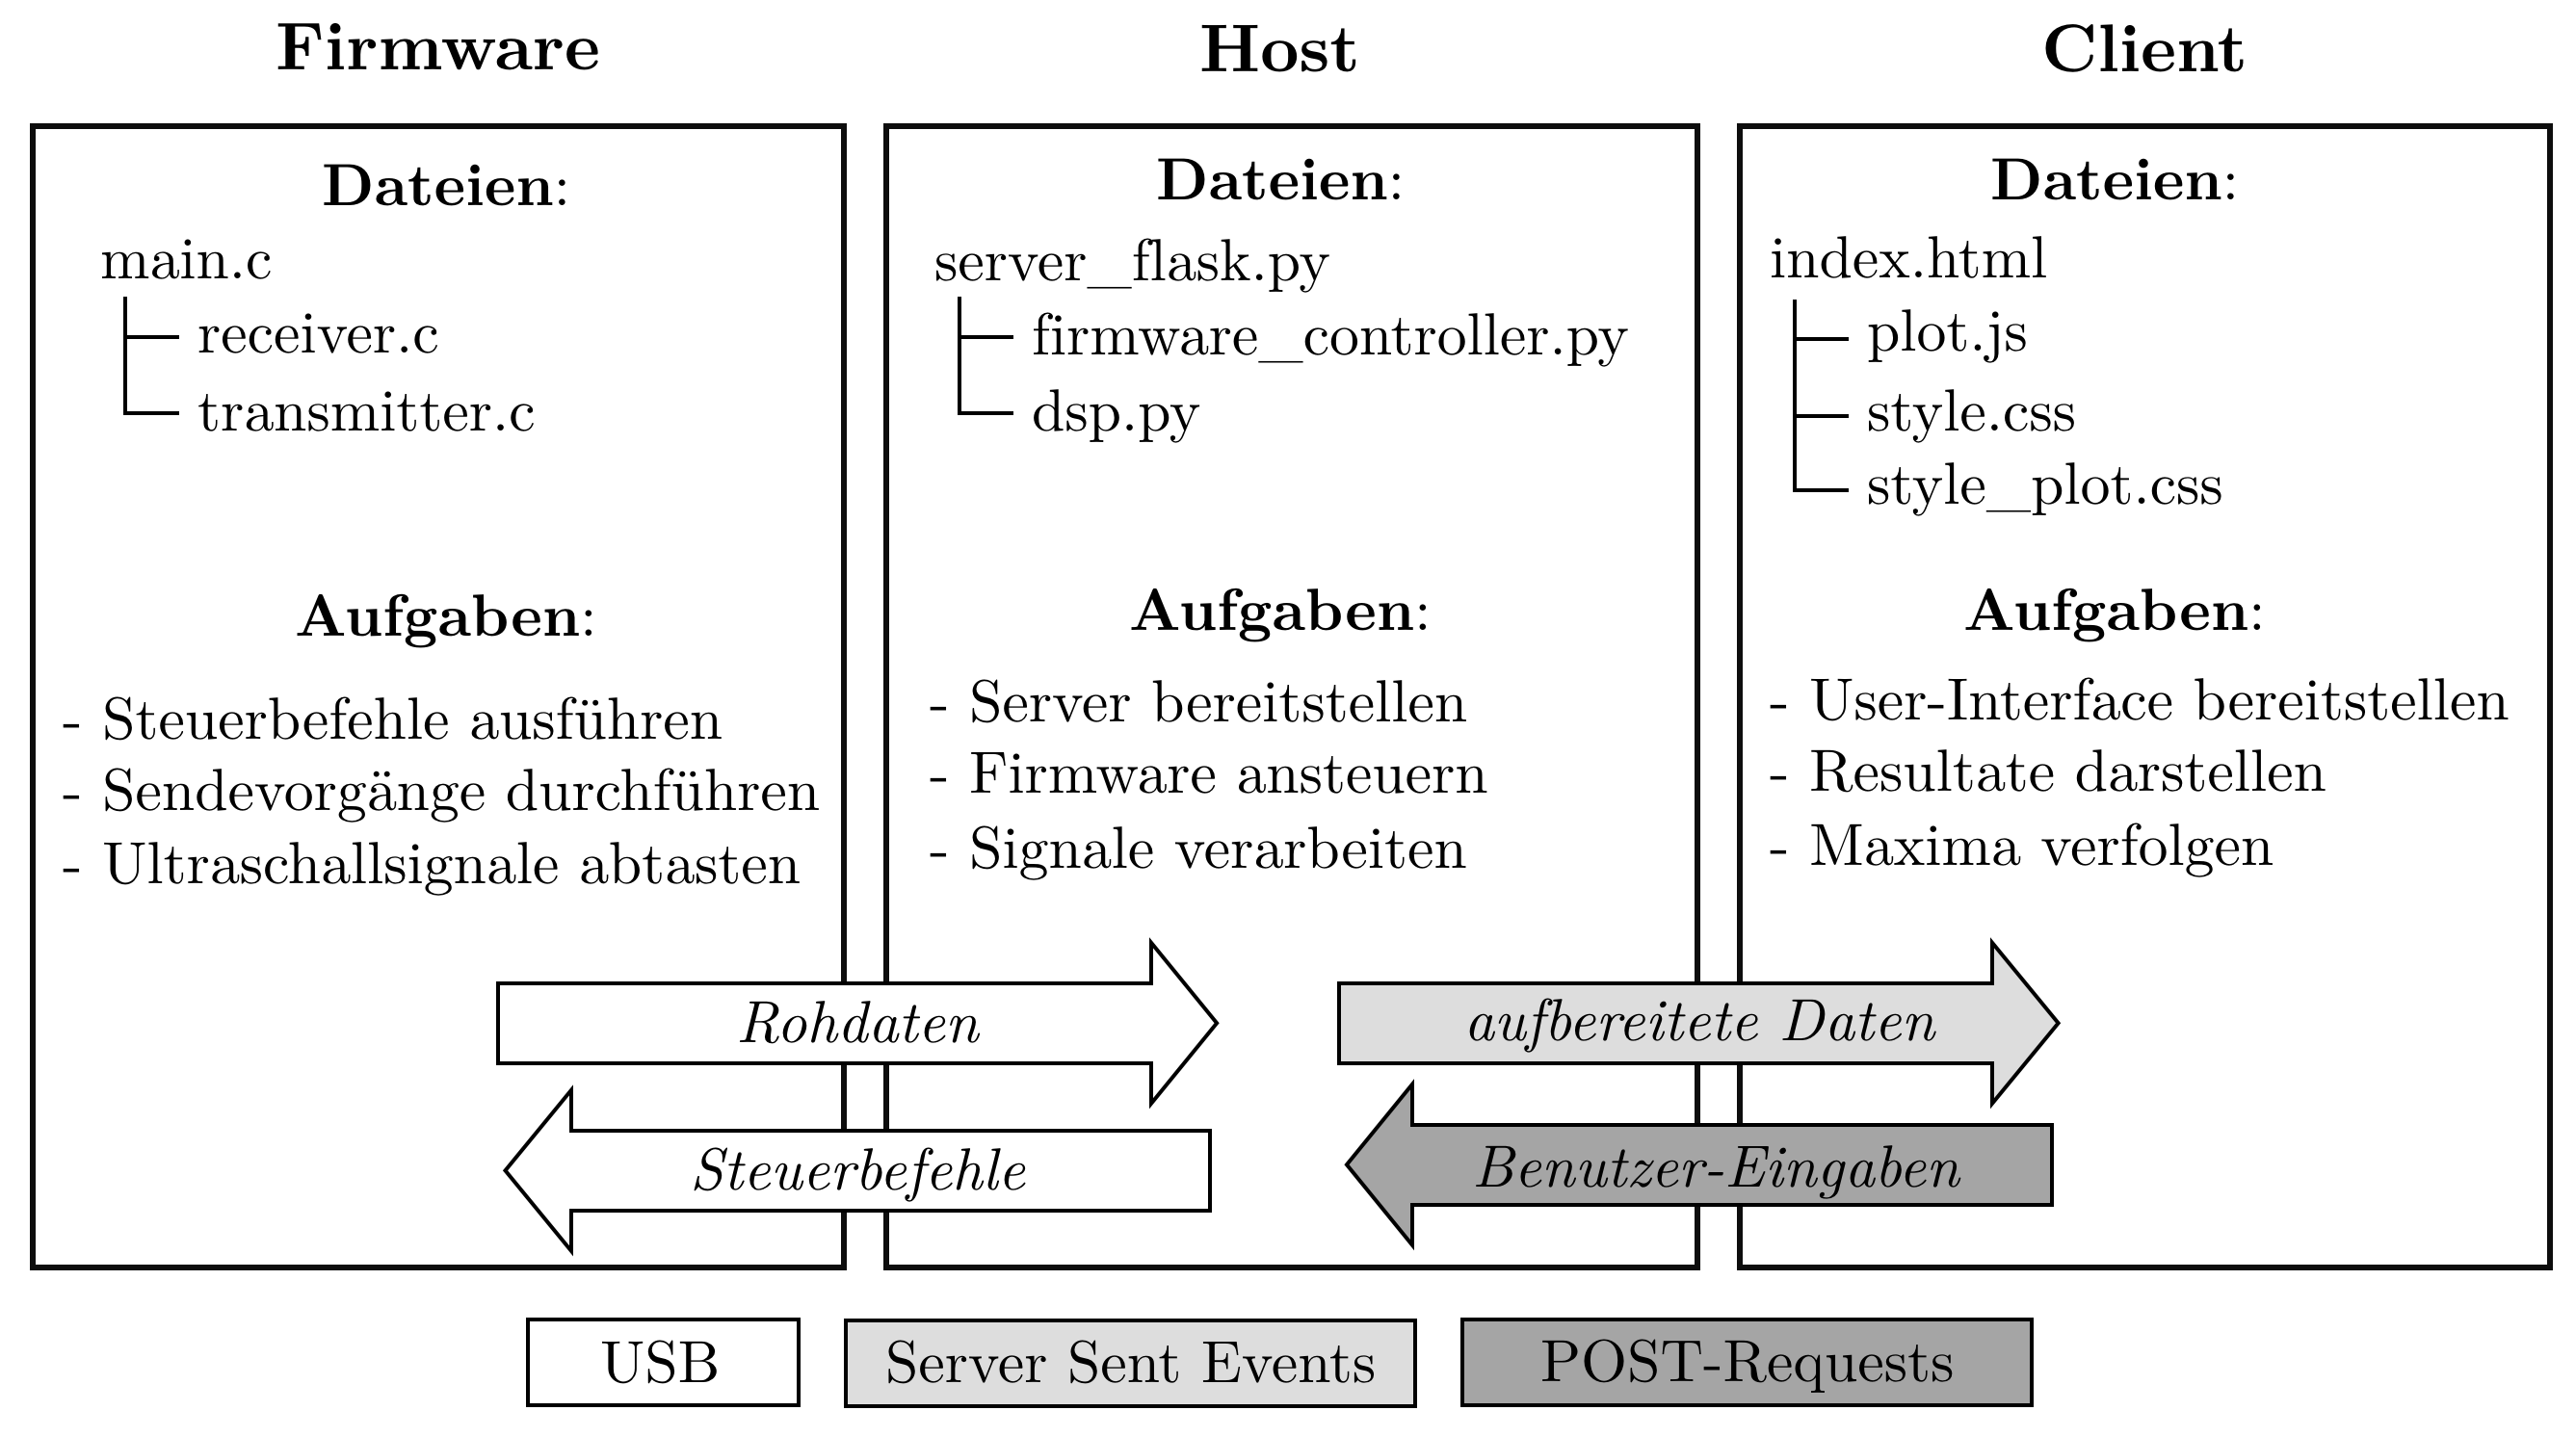
\includegraphics[width=\textwidth]{graphics/image_software_schema.png}
\end{center}
\caption{Gesamtübersicht Software} % picture caption
\label{fig:image_software_schema}
\end{figure}
%
%(Abb. \ref{fig:image1})
%%%%%%%%%%%%%%%%%%%%%%%%%%%%%%%%%%%%%%%%%%%%%%%%%%%%%%%%%%%%%%%%%%%%%%%%%%%%%%%%

Über die USB-Schnittstelle werden die Rohdaten der acht Ultraschallsignale an den Host übergeben. Dieser berechnet daraus (als Hintergrund-Thread des Webservers) das darzustellende Signal.
Server Sent Events sind eine HTML5-Technologie, welche es dem Client ermöglicht, asynchron Updates eines Servers zu erhalten. Somit kann der Webbrowser (Client) das darzustellende Signal zum jeweiligen Zeitpunkt seines Auftretens entgegennehmen und im User-Interface darstellen. Die Darstellung erfolgt als aktualisiertes Bild der Umgebung und als Linienplot.

Eingaben im User-Interface durch den Benutzer werden vom Server per POST-Request (auslesen eines Eingabeformulars auf der Webseite) vom Server übernommen. Diese Eingaben werden vom Host (als Hintergrund-Thread des Webservers) in  Steuerbefehle übersetzt, welche
die genauen Spezifikationen des nächsten Messvorgangs enthalten. Diese Steuerbefehle werden per USB an den Mikrocontroller übergeben. Dieser führt einen neuen Messvorgang aus und und sendet danach die neuen Rohdaten der acht Ultraschallsignale zurück.



%%%%%%%%%%%%%%%%%%%%%%%%%%%%%%%%%%%%%%%%%%%%%%%%%%%%%%%%%%%%%%%%%%%%%%%%%%%%%%%%
%%%%%%%%%%%%%%%%%%%%%%%%%%%%%%%%%%%%%%%%%%%%%%%%%%%%%%%%%%%%%%%%%%%%%%%%%%%%%%%%
%%%%%%%%%%%%%%%%%%%%%%%%%%%%%%%%%%%%%%%%%%%%%%%%%%%%%%%%%%%%%%%%%%%%%%%%%%%%%%%%
\subsection{Auswahl der Programmiersprachen und Schnittstellen}\label{sec:auswahl_der_programmiersprachen_und_schnittstellen}
Die Anforderungen an die Firmware auf dem Mikrocontroller erlauben dank der geringen Komplexität eine prozedurale Umsetzung in C. Ein Objektorientierter Ansatz in C++ ist nicht nötig.

Für die Umsetzung der Software auf dem Desktop-Betriebssystem (Signalverarbeitung und GUI) kommen zwei verschiedene Ansätze in Frage:

\begin{itemize}
	\item Standalone
	\item Server / Client
\end{itemize}

Wird die gesamte Software als Standalone-Anwendung geschrieben, hat dies eine geringere Komplexität zur Folge. Schnittstellen innerhalb der Software sind einfacher zu realisieren, im Vergleich zu den systemübergreifenden Schnittstellen einer Server-Client Realisierung.

Der Ansatz einer Webapplikation hat die Vorteile, dass die Rechenleistung zwischen Host und Client aufgeteilt werden kann. Zudem wird das User-Interface plattformunabhängig. So kann der Server z.B. auf einem Raspberry Pi betrieben werden und der Client über das lokale Netzwerk mittels Laptop auf den Server zugreifen. Damit wird das ganze Phased Array System mobil. Mit einem geeigneten Webframework ist der Mehraufwand im Vergleich zu einer Lösung, welche nur auf einem System umgesetzt ist klein.

Folgende drei Programmiersprachen kommen für die Implementation der serverseitigen Software in Frage und werden nachfolgend gegeneinander abgewogen.

\begin{itemize}
	\item C / C++
	\item Java
	\item Python
\end{itemize}

Eine sorgfältige Realisierung in C oder C++ ist bezüglich Performance kaum zu übertreffen. Im Vergleich zu den anderen Programmiersprachen ist C / C++ jedoch auch mit der aufwändigsten Realisierung verbunden. Die relativ lange Laufzeit des Schalls hat eine Wartezeit zwischen den Messungen zur Folge. Dadurch entsteht ein Zeitfenster, welches so gross ist, das eine derart optimierte Signalverarbeitung nicht nötig ist.

Eine Umsetzung in Java ist im Vergleich mit Python mit mehr Aufwand verbunden, da die Software für das Projekt 5 in Python realisiert wurde. Die zu klärende Frage ist, ob durch die Umsetzung der Signalverarbeitung in Python zusätzliche Wartezeiten zwischen den Messungen entstehen, welche mit Java verhindert werden könnten.
Wartezeiten entstehen im Projekt 5 tatsächlich, sowohl durch die Darstellung, als auch durch die Signalverarbeitung. Nach ersten Versuchen zur Beschleunigung der Algorithmen kann die Signalverarbeitung mittels Upsampling im Frequenzbereich (siehe Kapitel \ref{sec:upsampling_im_frequenzbereich}) vervielfacht werden. Damit wird die Verarbeitung in Python schnell genug. Mithilfe der Berechnung der Enveloppe und anschliessendem Downsampling kann auch die Darstellung beschleunigt werden. Ein Server-Client Ansatz ermöglicht zusätzlich eine Auslagerung der zur Darstellung benötigten Rechenleistung auf ein anderes System.

Die bereits im Projekt 5 zur Signalverarbeitung in Python verwendeten Bibliotheken \texttt{numpy} und \texttt{scipy} sind sowohl effizient, wie auch praktisch in der Handhabung. Codefragmente zur USB-Kommunikation und zur Signalverarbeitung (Zeitverschiebung im Frequenzbereich) können vom P5 mit wenigen Änderungen übernommen werden.
Zusätzlich ist Python beliebt bei der serverseitigen Programmierung, weshalb diverse Webframeworks zur Verfügung stehen. Als Python-Webframework bietet sich Flask als gut dokumentierte Alternative zum verbreiteten Django an. Flask ist wesentlich einfacher in der Handhabung und ein einfaches Webapp kann ohne grossen Aufwand aufgesetzt werden.
Server Sent Events ermöglichen es, dass der Client die darzustellenden Daten asynchron erhält und nicht ständig prüfen muss, ob neue Daten vorhanden sind.


\clearpage
%%%%%%%%%%%%%%%%%%%%%%%%%%%%%%%%%%%%%%%%%%%%%%%%%%%%%%%%%%%%%%%%%%%%%%%%%%%%%%%%
%%%%%%%%%%%%%%%%%%%%%%%%%%%%%%%%%%%%%%%%%%%%%%%%%%%%%%%%%%%%%%%%%%%%%%%%%%%%%%%%
%%%%%%%%%%%%%%%%%%%%%%%%%%%%%%%%%%%%%%%%%%%%%%%%%%%%%%%%%%%%%%%%%%%%%%%%%%%%%%%%
\subsection{Firmware auf dem Mikrocontroller}\label{sec:firmware_auf_dem_mikrocontroller}
Die Firmware auf dem Mikrocontroller steuert das Ultraschall Phased Array auf der entwickelten Hardware. Der Sourcecode kann in drei Module aufgeteilt werden. Diese werden nachfolgend kurz beschrieben. Neben dem Modul ''main.c'', welches das Hauptprogramm beinhaltet, gibt es die Module ''receiver.c'' und ''transmitter.c'', wobei sich diese Namen auf das Aussenden und Empfangen der Ultraschallsignale beziehen.

\subsubsection{Initialisierung und Hauptprogrammfluss -- main.c}\label{sec:initialisierung_und_hauptprogrammfluss}

Abbildung \ref{fig:image_software_microcontroller} zeigt die Initialisierung und den Hauptprogrammfluss der Firmware auf dem Mikrocontroller. Die Initialisierung ist als Ablaufdiagramm und die Statemachine als Zustandsdiagramm dargestellt.

%%%%%%%%%%%%%%%%%%%%%%%%%%%%%%%%%%%%%%%%%%%%%%%%%%%%%%%%%%%%%%%%%%%%%%%%%%%%%%%%
% pictures
\begin{figure}[htb]
\begin{center}
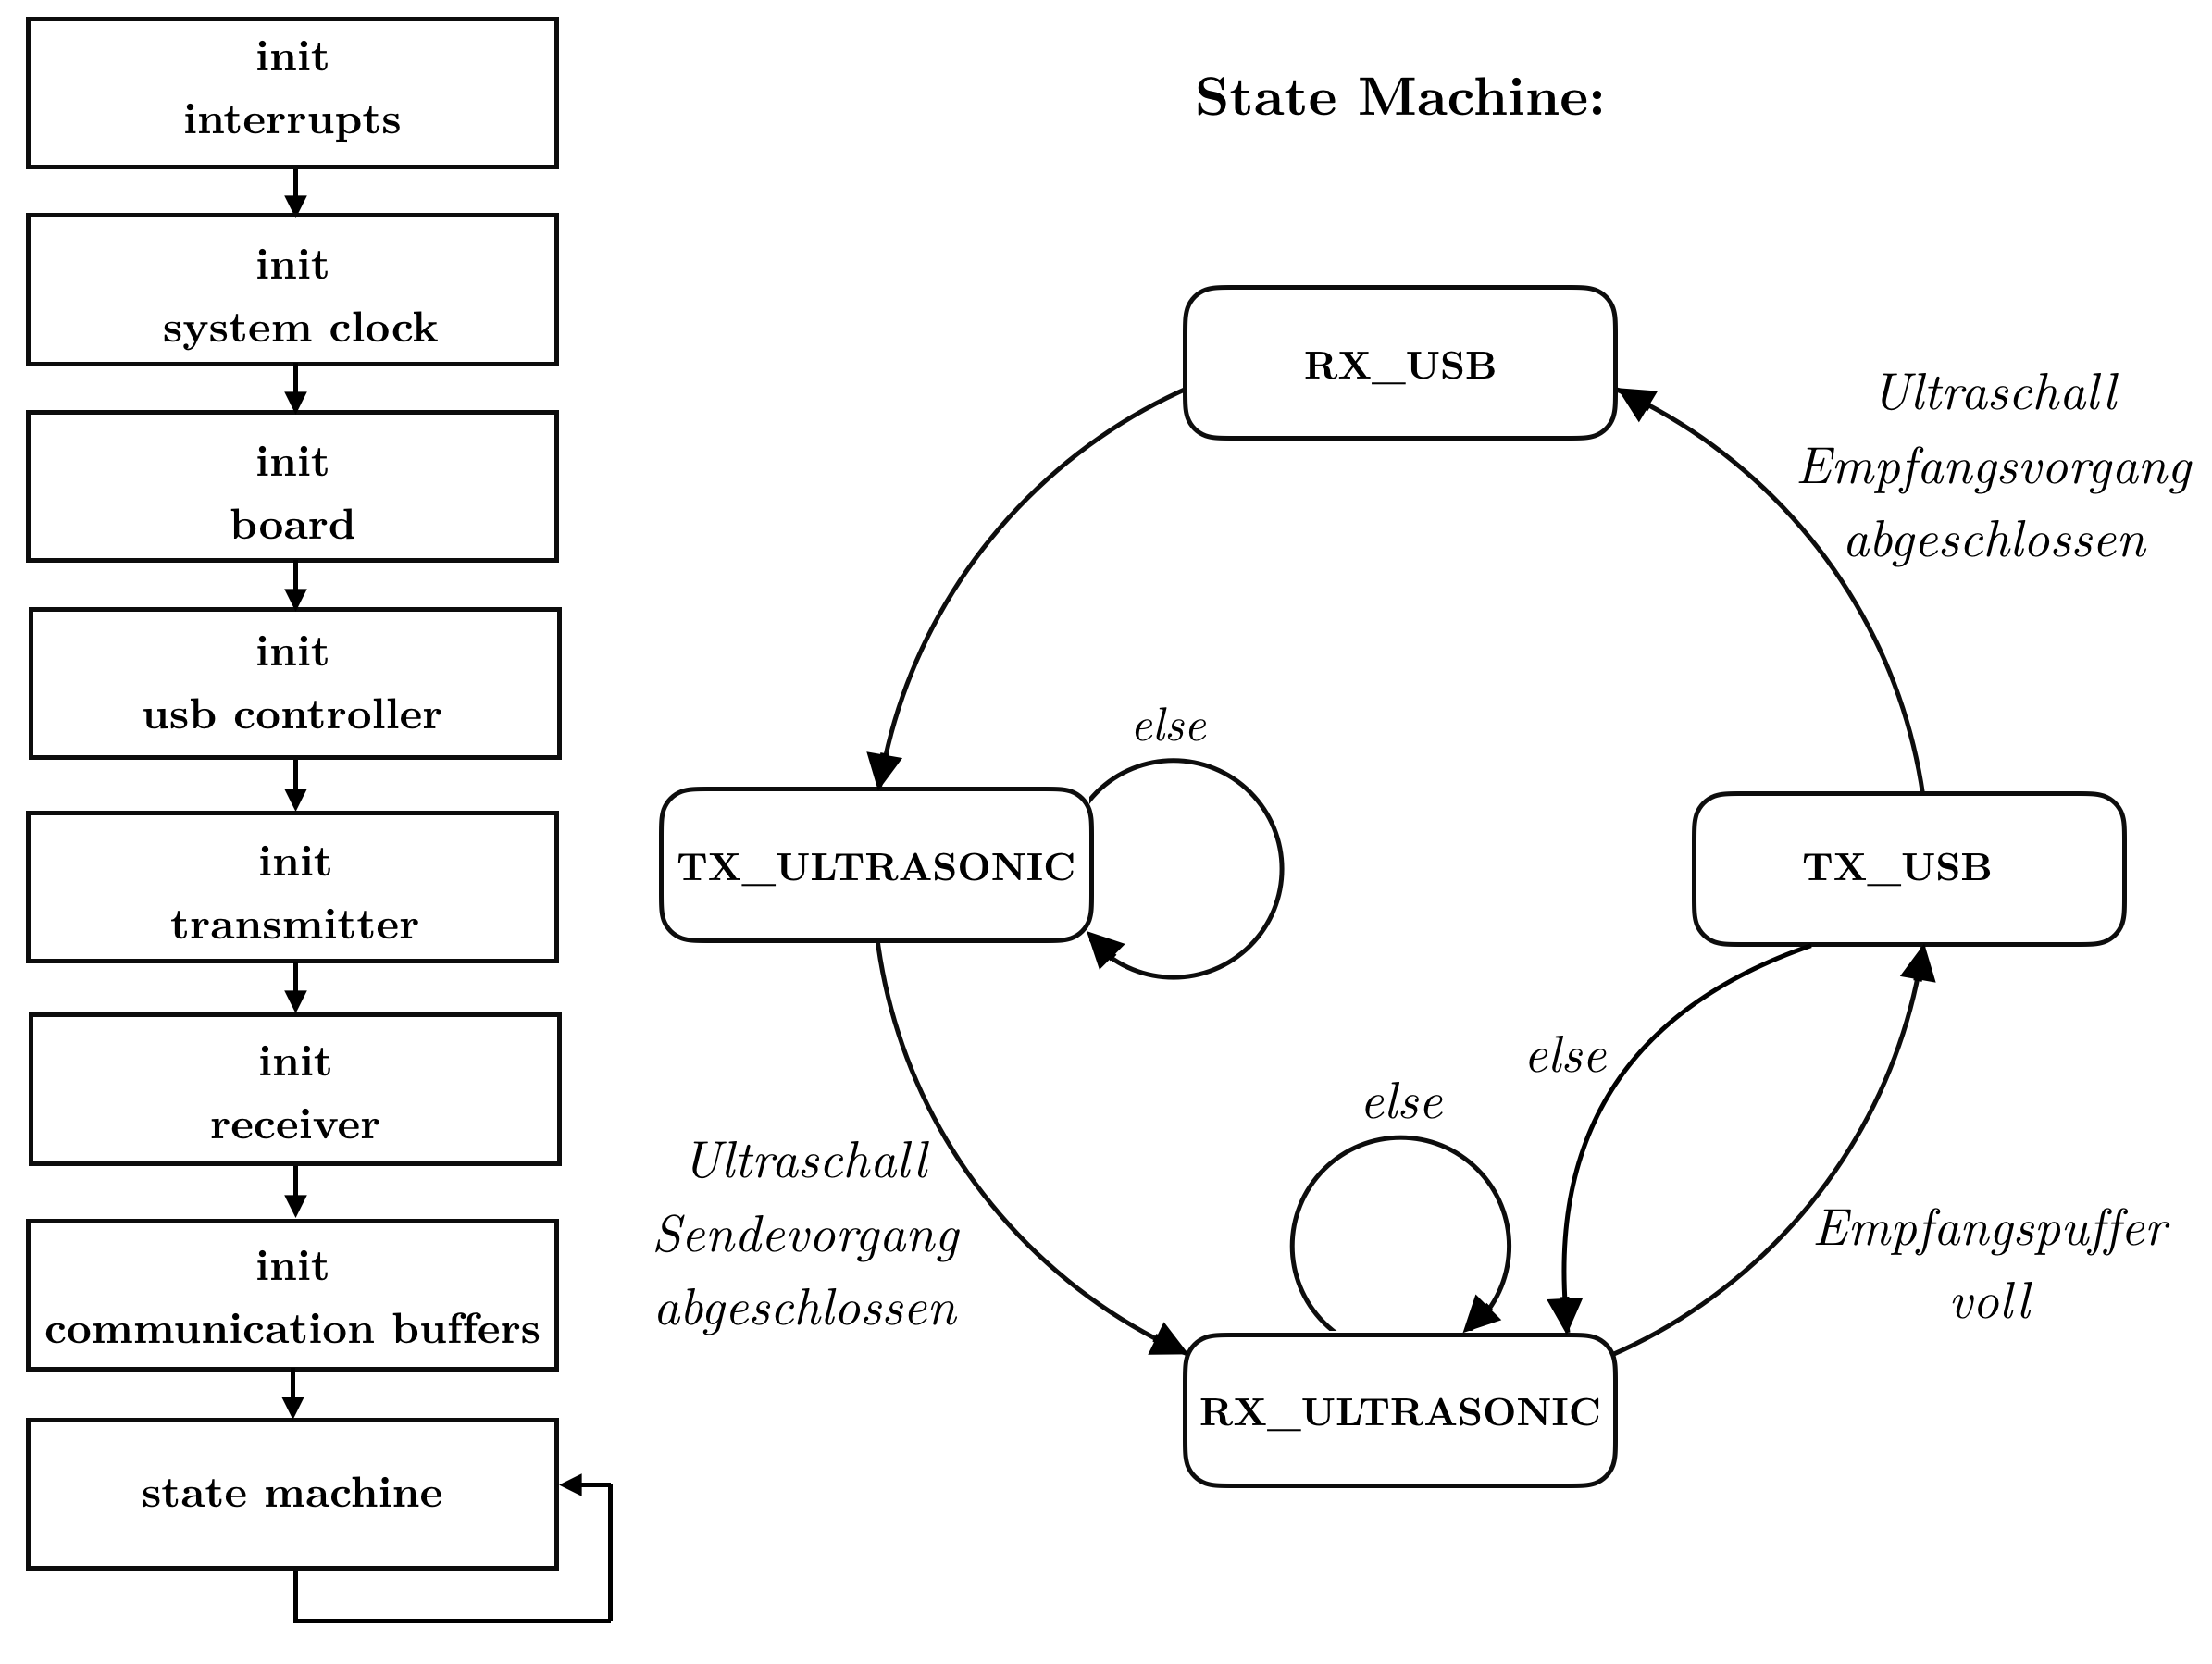
\includegraphics[width=\textwidth]{graphics/image_software_microcontroller.png}
\end{center}
\caption{Hauptprogrammfluss der Software auf dem Mikrocontroller} % picture caption
\label{fig:image_software_microcontroller}
\end{figure}
%
%(Abb. \ref{fig:image1})
%%%%%%%%%%%%%%%%%%%%%%%%%%%%%%%%%%%%%%%%%%%%%%%%%%%%%%%%%%%%%%%%%%%%%%%%%%%%%%%%

In der Initialisierung werden als erstes alle Treiber und Module konfiguriert, anschliessend wird in einer Endlosschlaufe die Statemachine aufgerufen. Diese unterscheidet vier verschiedene Zustände, welche in folgender Auflistung näher beschrieben sind.

\begin{itemize}
	\item\textbf{\texttt{RX\_USB:}} Dies ist der erste State nach dem Initialisierungsvorgang und als einziger ein blockierender State. In einer Endlosschlaufe wird gewartet, bis per USB ein Kontrollpuffer vom Host an die Firmware geschickt wurde. Nach Erhalt eines Puffers werden die darin enthaltenen Einstellungen extrahiert. Dies sind der aktuelle Sendewinkel, die gewünschte Amplitudenbelegung, die Anzahl Pulse mit welcher der Ultraschalltransceiver angeregt wird und die Anzahl der Datenpuffer, welche während dem Empfangsvorgang zu füllen sind. Danach wird falls nötig das Ultraschall Sendemodul mit den neuen Einstellungen initialisiert und in den State \texttt{TX\_ULTRASONIC} gewechselt.

	\item\textbf{\texttt{TX\_ULTRASONIC:}} Während diesem State werden Ultraschallsignale gesendet. Dies geschieht per PWM (Pulsweitenmodulation). Dieser State bleibt solange aktiv, bis die Funktion \texttt{transmitter\_send(int angle)} aus dem Modul ''transmitter.c'' per Rückgabewert signalisiert, dass der Sendevorgang abgeschlossen ist. Danach wird in den State \texttt{RX\_ULTRASONIC} gewechselt.

	\item\textbf{\texttt{RX\_ULTRASONIC:}} In diesem State werden vom ADC die empfangenen und verstärkten Ultraschallsignale abgetastet. Dabei werden Empfangspuffer gefüllt. Sobald ein Empfangspuffer voll ist, wird über den Rückgabewert der Funktion \texttt{receiver\_get\_buffer(int *receiver\_finished\_flag)} ein Pointer auf diesen Puffer übergeben. Dadurch wird in den State \texttt{TX\_USB} gewechselt. Solange der Rückgabewert hingegen ein \texttt{NULL}-Pointer ist wird im bisherigen State verblieben.

	\item\textbf{\texttt{TX\_USB:}} In diesem State werden die Empfangspuffer mit den vom ADC abgetasteten Werten per USB an den Host gesendet. Dabei wird pro ADC-Kanal ein USB-Puffer der Länge 1024 Bytes (512 16-Bit-Werte) gesendet. Vom USB-Stack werden diese Puffer in kleineren Teilstücken von 512 Bytes übermittelt, was aber auf die Statemachine keinen Einfluss hat. Ein zusätzlicher Puffer mit Statusinformationen wird als letztes gesendet. Danach wird anhand des im State \texttt{RX\_ULTRASONIC} gesetzten \texttt{receiver\_finished\_flag} entschieden, ob der Empfangsvorgang vollständig abgeschlossen ist und in den State \texttt{RX\_USB} gewechselt werden kann, oder ob im State \texttt{RX\_ULTRASONIC} auf weitere Empfangspuffer gewartet werden muss.
\end{itemize}


\subsubsection{Ultraschall Sender -- transmitter.c}\label{sec:ultraschall_sender}
Das Modul ''transmitter.c'' steuert die Senderschaltung des Ultraschall Phased Arrays. Dazu gehören die Levelshifter für die Verstärkung der Sendesignale und für das Dämpfen der Ultraschalltransceiver. Zusätzlich werden von diesem Modul auch die Analogschalter der Empfängerschaltung gesteuert.

Die einzelnen Kanäle des Levelshifters werden mit einem PWM-Signal der Frequenz $40 \mathrm{kHz}$ angesteuert. Um eine Richtwirkung zu erzielen, werden die PWM-Kanäle gegeneinander phasenverschoben betrieben. Dazu werden sie zeitlich verschoben eingeschaltet. Die Erzeugung dieser zeitlichen Verschiebung ist nicht ganz einfach, da sehr kleine Verschiebungen schon grosse Winkelveränderungen verursachen. Eine interruptgesteuerte Realisierung ist so zum Beispiel nicht möglich, da die Interrupt-Latenzzeit im Mikrosekundenbereich liegt, während die kleinste gewünschte Phasenverschiebung lediglich bei $\approx 250 \mathrm{ns}$ liegt. Aus diesem Grund wird auf eine relativ primitive Methode zurückgegriffen, bei welcher zwischen dem Einschalten der Kanäle eine winkelabhängige Anzahl Prozessortakte gewartet wird. Diese Wartezeit wird mithilfe von inline Assembler \texttt{nop} (no operation) Befehlen realisiert.

Der Ablauf des Sendevorgangs ist in einer Statemachine implementiert, welche zwischen den drei States \texttt{START}, \texttt{RUNNING} und \texttt{ATTENTUATE} unterscheidet. Zu Beginn des Sendevorgangs ist der State \texttt{START} aktiv. Sobald aus dem Hauptprogramm heraus die Funktion \texttt{transmitter\_send(int angle)} zum ersten Mal aufgerufen wird, werden die PWM-Kanäle eingeschaltet und der aktuelle State auf \texttt{RUNNING} gesetzt.

Während dem Senden muss für jeden Kanal gezählt werden, wie viele Pulse schon gesendet wurden. Da dies nicht so zeitkritisch ist wie das Einschalten, ist eine Implementation mithilfe einer Interrupt Routine möglich. Darin werden beim Erreichen der Maximalzahl Pulse die einzelnen PWM-Kanäle gleich ausgeschaltet. Nach dem Ausschalten des letzten Kanals wird der Dämpfungsvorgang gestartet und der State dementsprechend auf \texttt{ATTENTUATE} gewechselt.

Der Dämpfungsvorgang ist über einen Timer gesteuert. Sobald dieser Timer einen Schwellwert überschreitet, wird der Dämpfungsvorgang beendet, der State auf \texttt{START} gesetzt und dem Hauptprogramm mit dem Rückgabewert der Funktion \texttt{transmitter\_send(int angle)} mitgeteilt, dass der Sendevorgang beendet ist.

Neben dem Sendewinkel und der Anzahl zu sendender Ultraschallpulse kann auch die Amplitudenbelegung verändert werden. Eine Änderung der Spannungs- oder Stromamplitude an einem Ultraschalltransceiver hat eine Änderung der abgestrahlten Leistung zur Folge, welche quadratisch von der Amplitudenänderung abhängt. Da die Levelshifter in der Senderschaltung (siehe Kapitel \ref{sec:senderschaltung}) nicht einfach eine andere Spannung ausgeben können, wird die Sendeleistung mithilfe der Pulsbreite der PWM-Ansteuerung beeinflusst. Hier ist zu beachten, dass die abgestrahlte Leistung nicht quadratisch, sondern linear von der Pulsbreite abhängt. Die Werte für die Amplitudenbelegung müssen also im Quadrat mit der Pulsbreite multipliziert werden.


\subsubsection{Ultraschall Empfänger -- receiver.c}\label{sec:ultraschall_empfaenger}
Im Modul ''receiver.c'' werden die empfangenen analogen Ultraschallsignale digitalisiert. Dafür wird der interne Analog-Digital-Konverter (ADC) vom Mikrocontroller SAM3X8E eingesetzt. Für alle acht abzutastenden Kanäle steht lediglich ein einzelner ADC zur Verfügung. Dieser tastet demnach alle Kanäle in kurzen Abständen nacheinander ab. Dieses Verfahren nennt man Multiplexing und ist im Kapitel \ref{sec:multiplexing} näher beschrieben. Der gemessene zeitliche Abstand zwischen den Konversionen zweier benachbarter Kanäle beträgt $2 \mathrm{\mu s}$. Die daraus resultierende Phasenverschiebung bei einem $40 \mathrm{kHz}$-Signal ist zu gross, um sie vernachlässigen zu können. Während dem Upsampling auf dem Hostsystem wird sie korrigiert (siehe Kapitel \ref{sec:zeitverschiebung_im_frequenzbereich}).

Der Abtastvorgang der analogen Daten auf dem ADC des Mikrocontrollers läuft grösstenteils hardwaregesteuert ab. Als Trigger wird ein Hardware Timer verwendet. Dadurch ist die Abtastfrequenz konstant und wird nicht durch Interrupts beeinflusst. Beim interruptbasierten Triggern des ADC wurden teilweise Verzögerungen von mehr als $2 \mathrm{\mu s}$ gemessen, welche beim timerbasierten Triggern nicht auftreten.

Das Multiplexing findet mithilfe des ''Sequencer'' Modus statt. In diesem Modus werden sämtliche vorkonfigurierten ADC-Kanäle automatisch nacheinander konvertiert, sobald der ADC ge\-triggert wurde. Die abgetasteten Werte werden ebenfalls hardwaregesteuert vom DMA-Controller (Direct Memory Access) hintereinander in einen zuvor festgelegten Puffer gespeichert.

Der Ablauf eines Empfangsvorgangs sieht wie folgt aus: Aus der Statemachine im Hauptprogramm heraus wird einmalig die Funktion \texttt{receiver\_start(int bank\_count)} aufgerufen. Diese Funktion startet den ADC Trigger Timer. Der Übergabeparameter \texttt{bank\_count} legt fest, wie oft der Datenpuffer gefüllt werden soll bevor der Empfangsvorgang beendet wird. Die Statemachine im Hauptprogramm überprüft nun regelmässig über die Funktion \texttt{*receiver\_get\_buffer(int *stopped\_flag)}, ob ein neuer Datenpuffer gefüllt ist. Ist dies der Fall, liefert die Funktion einen Pointer auf den gefüllten Puffer, ansonsten einen \texttt{NULL}-Pointer. Die Variable \texttt{stopped\_flag} signalisiert den letzten Datenpuffer nachdem der Empfangsvorgang beendet wurde.

Insgesamt gibt es 4 Datenpuffer, welche alle gleich gross sind. Zwei davon werden als temporäre Puffer (\texttt{temp\_buffer}) bezeichnet, zwei als Empfängerpuffer (\texttt{receiver\_buffer}). Die zwei temporären Puffer werden vom DMA-Controller des ADC hardwaregesteuert beschrieben und in der ADC Interrupt Routine in die Empfängerpuffer umsortiert. Es wird jeweils ein Puffer beschrieben, während der andere ausgelesen wird, danach umgekehrt. Die beiden Empfängerpuffer werden in der ADC Interrupt Routine beschrieben und im Hauptprogramm vom USB-Controller ausgelesen. Auch hier werden die Puffer jeweils nach dem Schreiben/Lesen ausgetauscht.

Pro Kanal werden vom ADC per DMA je 512 Werte (16-Bit Integer) in die temporären Datenpuffer \texttt{temp\_buffer} gespeichert, demzufolge sind alle Puffer $512 \cdot 8 \cdot 2 \mathrm{B} = 8192 \mathrm{B}$ gross. Jedes Mal wenn der ADC vom Timer Trigger ausgelöst wird, schreibt er die Werte der 8 Kanäle der Reihe nach in den temporären Puffer. Bezeichnet man die Kanäle mit den Buchstaben a-h, sieht dieser Puffer demzufolge so aus:

$$\texttt{temp\_buffer[0]} = [a_{0}, b_{0}, c_{0}, d_{0}, e_{0}, f_{0}, g_{0}, h_{0}, a_{1}, b_{1}, \dots, a_{511}, b_{511}, c_{511}, d_{511}, e_{511}, f_{511}, g_{511}, h_{511}]$$

Sobald nun der erste Puffer voll ist, wird ein ADC Interrupt ausgelöst. In diesem Interrupt wird zunächst dem DMA-Controller des ADC der zweite temporäre Puffer übergeben. Danach wird der soeben gefüllte Puffer in einen der zwei Empfängerpuffer umsortiert. Nach dem Umsortieren stehen die Werte wie folgt in dem USB Empfängerpuffer:

$$\texttt{receiver\_buffer[0]} = [a_{0}, a_{1}, a_{2}, \dots, a_{510}, a_{511}, b_{0}, b_{1}, \dots, h_{510}, h_{511}]$$

Sobald ein Puffer umsortiert ist, wird dies dem Hauptprogramm über die oben schon erwähnte Funktion \texttt{*receiver\_get\_buffer(int *stopped\_flag)} mitgeteilt. Im Hauptprogramm wird dann der Puffer dem USB-Controller übergeben und an den Host gesendet. Das Umsortieren der Daten hat den Zweck, dass auf dem Host die Daten schon nach Kanal getrennt ankommen, so dass dort keine Rechenleistung mit Umsortieren verschwendet wird.


\clearpage
%%%%%%%%%%%%%%%%%%%%%%%%%%%%%%%%%%%%%%%%%%%%%%%%%%%%%%%%%%%%%%%%%%%%%%%%%%%%%%%%
%%%%%%%%%%%%%%%%%%%%%%%%%%%%%%%%%%%%%%%%%%%%%%%%%%%%%%%%%%%%%%%%%%%%%%%%%%%%%%%%
%%%%%%%%%%%%%%%%%%%%%%%%%%%%%%%%%%%%%%%%%%%%%%%%%%%%%%%%%%%%%%%%%%%%%%%%%%%%%%%%
\subsection{Hostseitige Software auf dem Desktop-Betriebssystem}\label{sec:hostseitige_software_auf_dem_desktop-betriebssystem}
Das Pythonpogramm übernimmt als Hauptaufgabe die Vermittlung zwischen User-Interface (Client) und Hardware (Firmware). Es stellt dafür einen Webserver zur Verfügung, verarbeitet Benutzereingaben und bereitet Rohdaten mittels Signalverarbeitung auf. Der Webserver ist mithilfe des Webframeworks Flask implementiert. Eine Übersicht des Programms ist in Abbildung \ref{fig:image_software_host_schema} dargestellt.

Das Hauptprogramm wird über das File ''server\_flask.py'' gestaratet. Es generiert eine Web\-appli\-kation bestehend aus Server und Applikation. Bei einem Client-Zugriff auf den Webserver wird auf dem Host eine zur aufgerufenen HTTP-Adresse zugehörige Python-Funktion ausgeführt. So wird z.B. beim Aufruf der Adresse \texttt{http://address:5000/} die Funktion \texttt{index()} aufgerufen. Diese Funktion erzeugt dynamischen HTML-Code für das GUI, welcher daraufhin zur Ausführung an den Client (Webbrowser) übergeben wird. Näheres zum clientseitigen Code ist im Kapitel \ref{sec:clientseitige_software_auf_dem_desktop_betriebssystem} zu finden.
Die Applikation startet zudem den Firmware Controller, welcher als Instanz der Klasse \texttt{FirmwareController} in einem eigenen Thread ausgeführt wird. Dieser kommuniziert über USB mit der Hardware und verarbeitet die Rohdaten mithilfe statischer Methoden aus der Klasse \texttt{DSP}.

%%%%%%%%%%%%%%%%%%%%%%%%%%%%%%%%%%%%%%%%%%%%%%%%%%%%%%%%%%%%%%%%%%%%%%%%%%%%%%%%
% pictures
\begin{figure}[htb]
\begin{center}
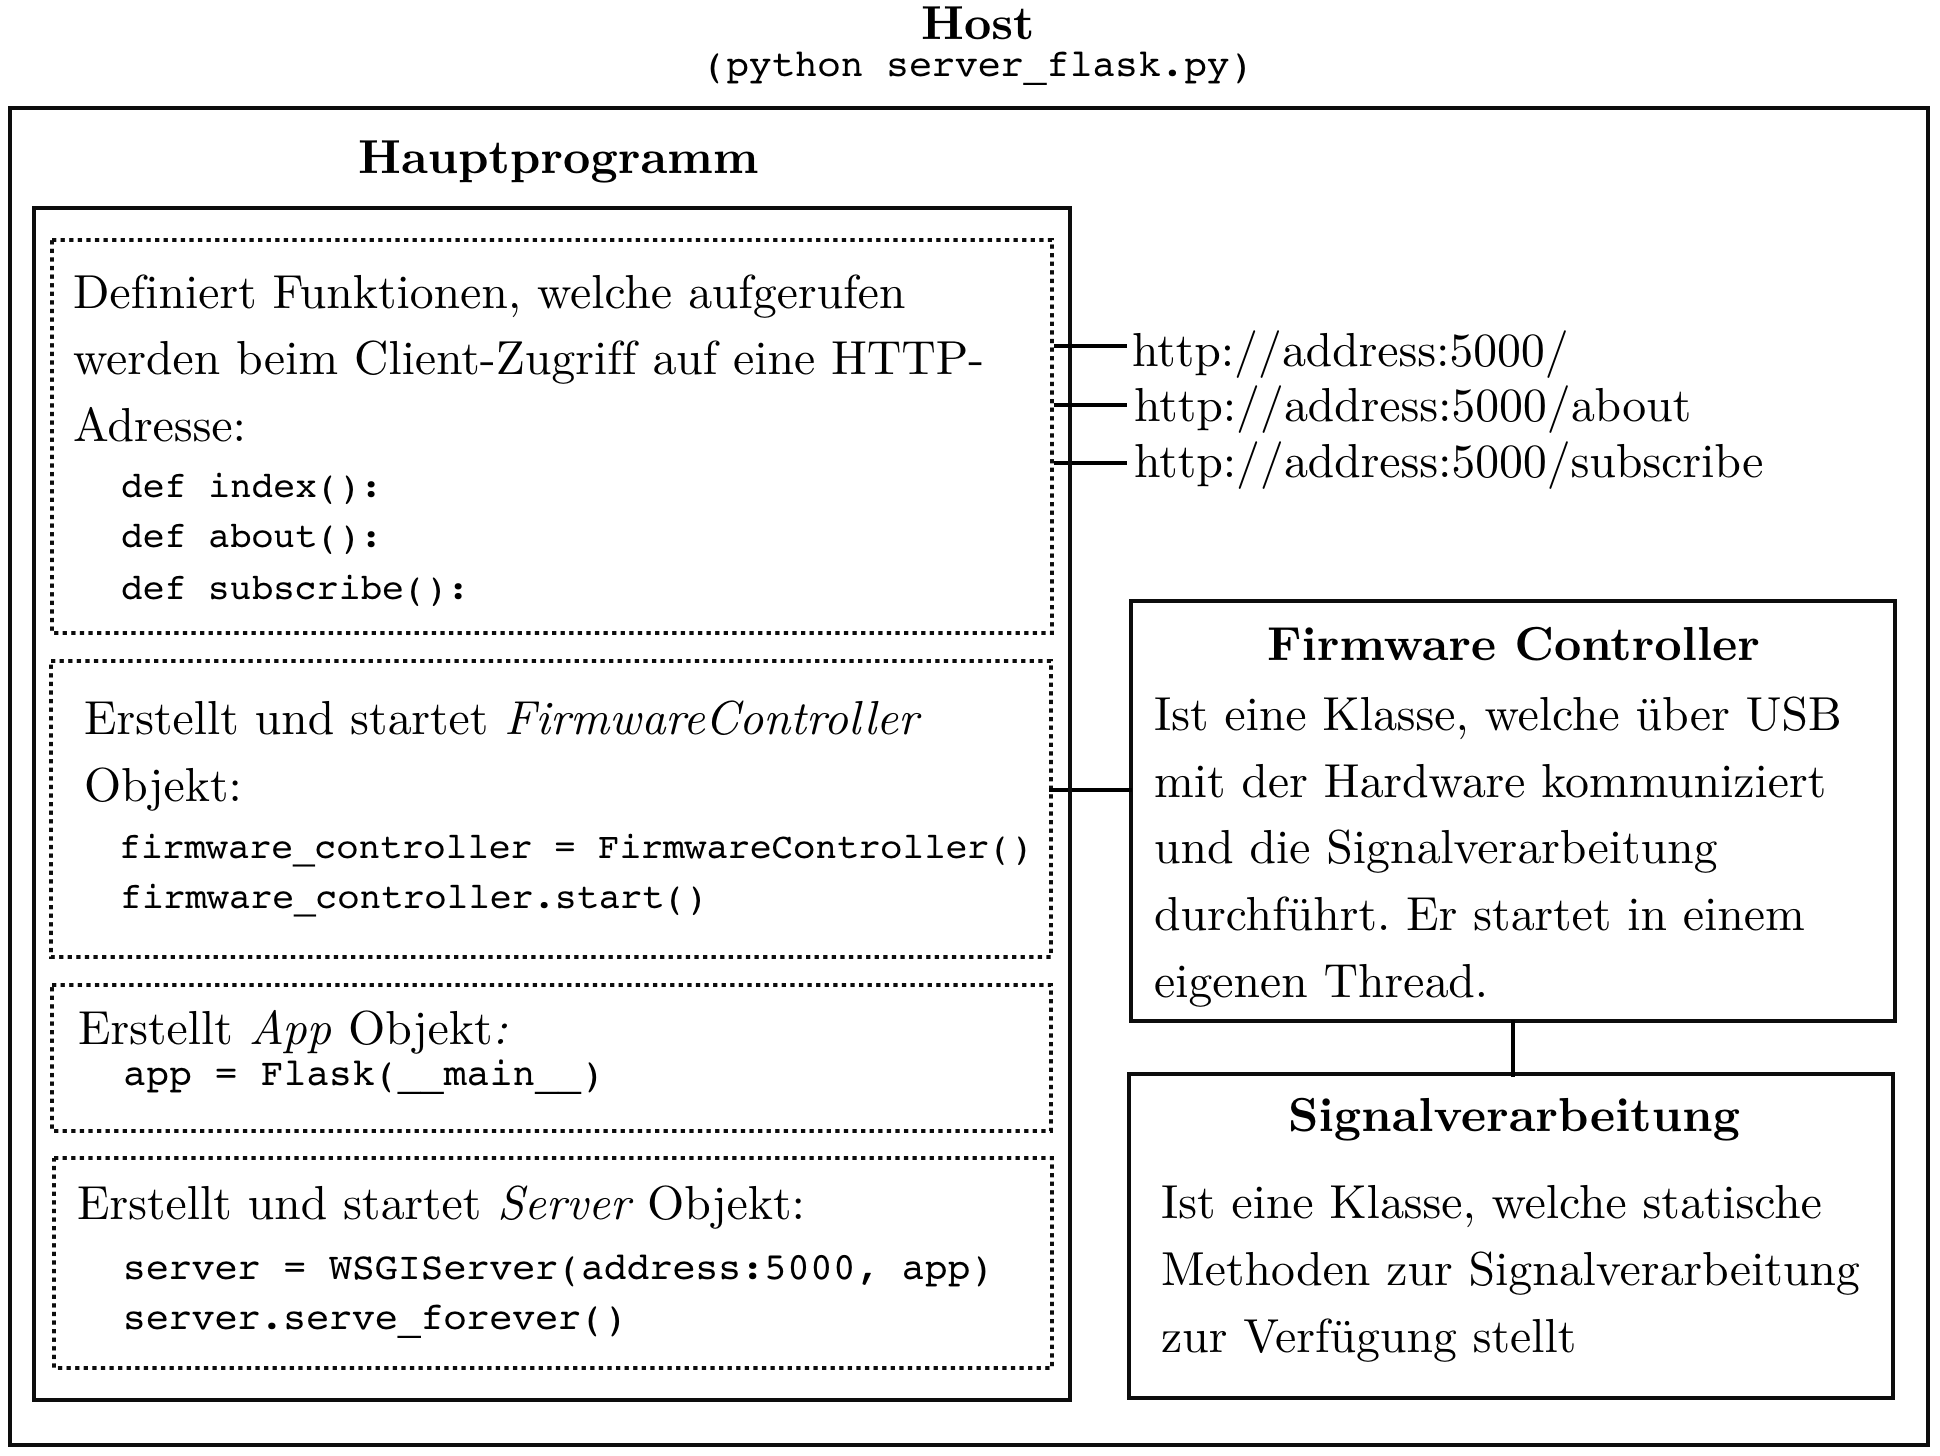
\includegraphics[width=\textwidth]{graphics/image_software_host_schema.png}
\end{center}
\caption{Übersicht Host} % picture caption
\label{fig:image_software_host_schema}
\end{figure}
%
%(Abb. \ref{fig:image1})
%%%%%%%%%%%%%%%%%%%%%%%%%%%%%%%%%%%%%%%%%%%%%%%%%%%%%%%%%%%%%%%%%%%%%%%%%%%%%%%%


\clearpage
\subsubsection{Hauptprogramm -- server\_flask.py}\label{sec:hauptprogramm}
Flask ist ein BSD lizensiertes, kleines Webframework, welches es ermöglicht, mit wenigen Zeilen Code eine Webapplikation zu erstellen. Das Web Server Gateway Interface (WSGI) ist eine Schnittstellenspezifikation für die Kommunikation zwischen einer Python-Applikation und dem Server. Flask generiert WSGI-konforme Apps, welche folglich von WSGI-kompatiblen Servern ausgeführt werden können. Als Server wird der WSGI-Server der Bibliothek \texttt{Gevent} verwendet.

Wie in Abbildung \ref{fig:image_software_host_schema} ersichtlich, wird beim Client-Zugriff auf eine HTTP-Adresse eine zugehörige Python Funktion ausgeführt. Es wird zwischen folgenden drei Funktionen unterschieden:

\begin{itemize}
	\item \texttt{index() : http://adress:5000}
	\item \texttt{about()  : http://adress:5000/about}
	\item \texttt{subscribe() : http://adress:5000/subscribe}
\end{itemize}

Die Funktion \texttt{index()} generiert den HTML-Code für das GUI auf der Basis eines HTML-Templates (siehe Kapitel \ref{sec:html_und_css}). Es werden dafür die Eingabefelder des GUIs ausgelesen und die aktualisierten Benutzereingaben an den Firmware Controller übergeben. Da das Hauptprogramm über ein Firmware Controller Objekt verfügt, ist dies mithilfe der Funktion \texttt{firm\-ware\_con\-troller.update\_values(\dots)} möglich. Mit der Flask-Funktion \texttt{ren\-der\_temp\-late(html\-\_temp\-late, python\_variables)} wird der HTML Code generiert. Dieser Funktion werden als Python-Variablen Eingabefelder (HTML kompatibel) mit den aktualisierten Werten mitgegeben.

Die Funktion \texttt{about()} generiert statischen HTML-Code mit Informationen über das Projekt.

Über die Funktion \texttt{subscribe()} abonniert der Client die asynchronen Updates, welche jeweils das darzustellende Signal mit dazugehörigen Informationen enthalten. Dafür werden Server Sent Event Objekte mit den neuen Daten aus dem Firmware Controller erstellt und an den Client übertragen.

Damit diese asynchrone Schnittstelle möglich wird, verfügt die Applikation über ein Interface Objekt. Dieses aktualisiert sich über eine Callback-Funktion, welche vom Firmware Controller aufgerufen wird, sobald neue Daten vorhanden sind. Das Hauptprogramm hat über die Funktion \texttt{interface.get\_data()} Zugriff auf die darzustellenden Ultraschallsignale.

Flask erstellt aus dem Source-Code eine WSGI-konforme Applikation. Mit dieser wird daraufhin der WSGI-Server erstellt, welcher schlussendlich gestartet wird (siehe Abbildung \ref{fig:image_software_host_schema}).


\subsubsection{Firmware Controller -- firmware\_controller.py}\label{sec:firmware_controller}
Der Firmware Controller vermittelt zwischen der Flask-Applikation und der Firmware auf dem Arduino. Er erstellt dabei aus Benutzereingaben, welche in der Flask-Applikation gespeichert sind, Steuerbefehle für den Arduino. Umgekehrt bearbeitet er vom Arduino kommende Rohdaten, sodass sie zur Darstellung bereit sind und übergibt diese der Applikation. Eine Übersicht der hostseitigen Software aus der Perspektive des Firmware Controllers ist in Abbildung \ref{fig:image_software_firmware_controller} zu sehen.

%%%%%%%%%%%%%%%%%%%%%%%%%%%%%%%%%%%%%%%%%%%%%%%%%%%%%%%%%%%%%%%%%%%%%%%%%%%%%%%%
% pictures
\begin{figure}[htb]
\begin{center}
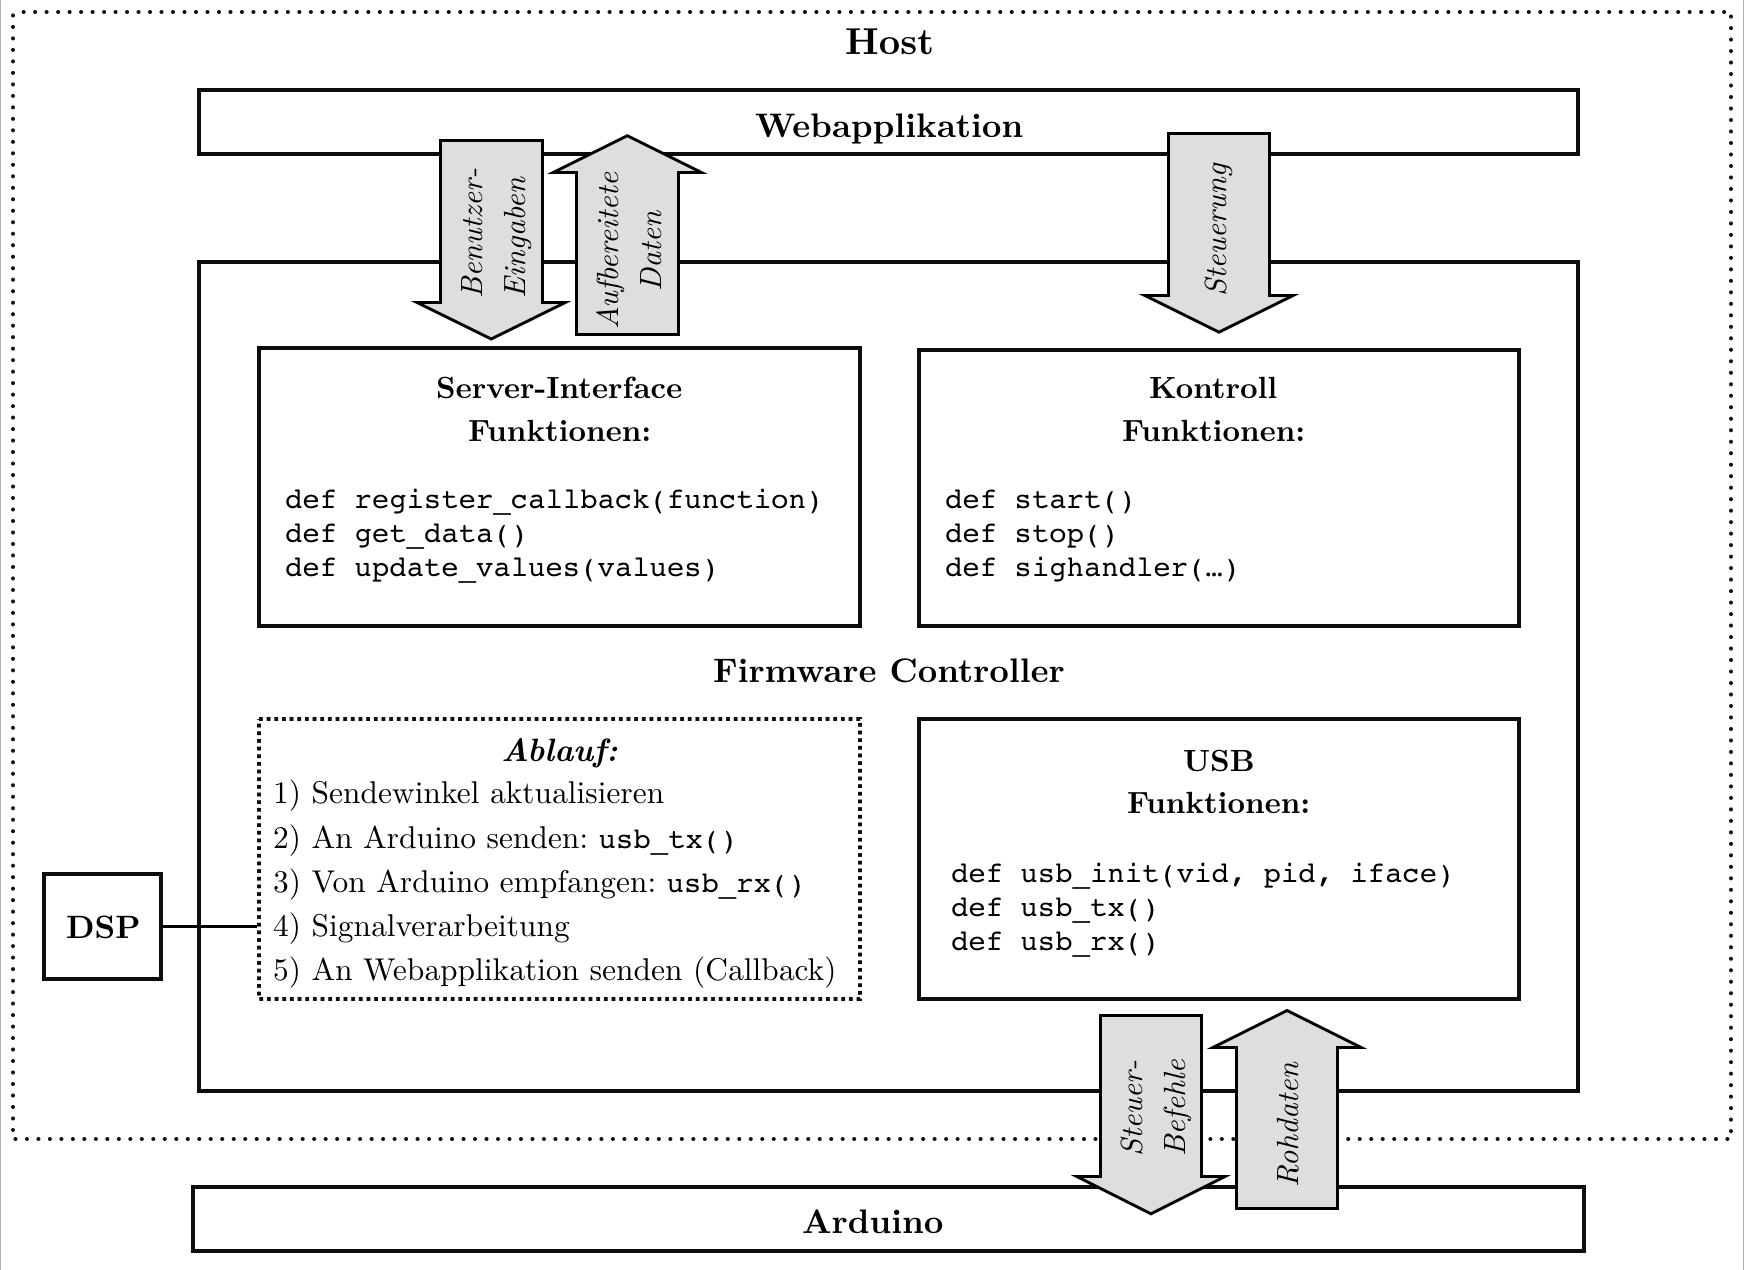
\includegraphics[width=\textwidth]{graphics/image_software_firmware_controller.png}
\end{center}
\caption{Die Hostsoftware aus der Perspektive des Firmware Controllers} % picture caption
\label{fig:image_software_firmware_controller}
\end{figure}
%
%(Abb. \ref{fig:image1})
%%%%%%%%%%%%%%%%%%%%%%%%%%%%%%%%%%%%%%%%%%%%%%%%%%%%%%%%%%%%%%%%%%%%%%%%%%%%%%%%

Das File ''firmware\_controller.py'' enthält eine Klassendeklaration, die vom Hauptprogramm (Flask-Applikation) genau einmal instanziert wird. Über dieses \texttt{FirmwareController} Objekt kommuniziert die Flask-Applikation mit dem Arduino (siehe Abbildung \ref{fig:image_software_host_schema}).

Für den Firmware Controller wird ein eigener Thread gestartet, damit er seine Aufgaben parallel zur Flask-Applikation ausführen kann. Seine Hauptaufgabe führt der Firmware Controller dabei über die Funktion \texttt{main\_loop()} aus, welche in einer Endlosschleife ausgeführt wird (''Ablauf'' in der Abbildung \ref{fig:image_software_firmware_controller}).
Der Sendewinkel ist als globale Variable \texttt{angle} im Firmware Controller gespeichert. Vor jedem neuen Zyklus der Endlosschleife wird dieser Sendewinkel inkrementiert oder auf den Startwinkel zurückgesetzt, sodass der im GUI eingestellte Winkelbereich durchlaufen wird. Danach wird der neue Messvorgang für diesen Winkel ausgelöst und die entsprechenden Rohdaten der Ultraschallsignale entgegengenommen. Das darzustellende Signal wird mithilfe der Methoden aus der \texttt{DSP} Klasse (siehe \ref{sec:signalverarbeitung}) aus diesen Rohdaten berechnet. Schlussendlich wird das Signal (und weitere Informationen) mithilfe einer Callback-Funktion an die Flask-Applikation übergeben.

Die restlichen Funktionen im Firmware Controller sind anhand ihrer Zuständigkeit grob in drei Bereiche unterteilt (siehe Abbildung \ref{fig:image_software_firmware_controller}):

\begin{itemize}
	\item Kontroll-Funktionen
	\item USB-Funktionen
	\item Server-Interface-Funktionen
\end{itemize}

Die \textit{Kontroll-Funktionen} sind für das Starten und Beenden des Firmware Controllers verantwortlich. Mit der Funktion \texttt{firmware\_controller.start()} wird das USB-Interface initialisiert, ein eigener Thread gestartet und Keyboardinterrupt-Signale abgefangen. Danach beginnt der Controller im neuen Thread seine Hauptaufgabe (\texttt{main\_loop()}).
Wenn der Server aus der Shell mit Ctrl-C beendet wird, wird der Firmware Controller mit der Funktion \texttt{stop()} beendet. Diese Funktion beendet den Thread des Firmware Controllers.

Für die Kommunikation mit dem Arduino sind \textit{USB-Funktionen} implementiert. Nachdem das USB-Interface mithilfe der Funktion \texttt{usb\_init(vid, pid, iface)} initialisiert ist, kann mit der Funktion \texttt{usb\_tx()} ein Messvorgang auf der Firmware (Arduino) gestartet werden. Der Firmware Controller hat die aktuellsten Eingaben aus dem User-Interface und den aktuellen Sendewinkel gespeichert. Mit diesen Variablen ist der auszuführende Messvorgang spezifiziert. Da innerhalb der Funktion \texttt{usb\_tx()} direkt auf diese Variablen zugegriffen wird, benötigt die Funktion keine Übergabewerte. Mit der Funktion \texttt{usb\_rx()} werden die Rohdaten der gemessenen Ultraschallsignale entgegengenommen. Die im GUI ausgewählte Anzahl Puffer bestimmt dabei die Grösse (Signallänge) der empfangenen USB-Daten.

Die \textit{Server-Interface-Funktionen} sind für die Kommunikation zwischen der Flask-Applikation und dem Firmware Controller zuständig. Die Flask-Applikation übergibt die aktuellen Benutzereingaben mithilfe der Funktion \texttt{firmware\_controller.update\_values(\dots)} dem Firmware Controller.
Über die Funktion \texttt{firmware\_controller.register\_callback(callback\_function)} speichert die Flask-Applikation eine Funktion im Firmware Controller, welche jeweils sofort nach der Signalverarbeitung ausgeführt wird. Bei dieser von der Flask-Applikation übergebenen Funktion handelt es sich um \texttt{firmware\_controller.get\_data()}. Damit werden die asynchronen Updates zwischen Client und Host ausgelöst (siehe Kapitel \ref{sec:hauptprogramm}).

\subsubsection{Signalverarbeitung -- dsp.py}\label{sec:signalverarbeitung}
Echos von Objekten im Umfeld des Phased Arrays kommen mit zeitlichen Verzögerungen bei den acht Ultraschall Empfängern an. Durch die Auswertung dieser Verzögerungen können Informationen über Distanz und Winkel dieser Objekte berechnet werden. Aus den Rohdaten der acht Signale wird ein einzelnes Signal berechnet, welches anzeigt, aus welcher Distanz Echos aus einem bestimmten Winkel stammen.
Dieses Signal wird im User-Interface dargestellt.

Im Kapitel \ref{sec:digitale_signalverarbeitung} ist die dazugehörige Theorie zusammengefasst. Die Rohdaten durchlaufen der Reihe nach folgende Verarbeitungsschritte:

\begin{itemize}
	\item 1: Upsampling
	\item 2: Beamforming
	\item 3: Enveloppe berechnen
	\item 4: Downsampling
\end{itemize}

Die Klasse \texttt{DSP} stellt die dafür nötigen Signalverarbeitungs-Methoden als statische Funktionen zur Verfügung. Diese Klasse ist im File ''dsp.py'' deklariert und wird vom Firmware Controller importiert. Es werden für die Berechnungen Funktionen aus den open source Bibliotheken \texttt{numpy} und \texttt{scipy} verwendet. Die Signalverarbeitung ist unterteilt in folgende drei Funktionen:

\begin{itemize}
	\item \texttt{get\_aperture(aperture, max\_n)}
	\item \texttt{upsamp\_beam\_form(y, phi\_rad, aperture, sonic\_speed, upsample\_factor)}
	\item \texttt{downsamp\_env(y, downsample\_factor)}
\end{itemize}

Die Funktion \texttt{get\_aperture(aperture, max\_n)} berechnet die im Kapitel \ref{sec:amplitudenbelegung} beschriebenen Gewichtungsfaktoren der Amplitudenbelegung für \texttt{max\_n} Elemente. Der Übergabeparameter \texttt{aperture} wird als Integer erwartet. Es kann zwischen Rechteckbelegung ($0$), $\cos$-Belegung ($1$), $\cos^{2}$-Belegung ($2$) und Gauss\-belegung ($3$) ausgewählt werden. Als Resultat wird eine Python-Liste mit den berechneten Werten zurückgegeben.

Die Funktion \texttt{upsamp\_beam\_form(y, phi\_rad, aperture, sonic\_speed, upsample\_factor)} erhöht die Abtastrate der unterabgetasteten Rohdaten um den Faktor \texttt{upsample\_factor} (siehe Kapitel \ref{sec:upsampling}). Falls gewünscht, werden die Signale mit einer Amplitudenbelegung versehen (siehe Kapitel \ref{sec:amplitudenbelegung}). Schlussendlich werden die Signale mittels Beamforming (siehe Kapitel \ref{sec:beamforming}) zu einem Signal addiert, welches eine empfangsseitige Richtwirkung in die Senderichtung aufweist.
Die Funktion übernimmt als Eingabeparameter die acht unterabgetasteten Signale der Ultraschalltransceiver \texttt{y} als $1$x$8$ Python-Liste. Zusätzlich wird der Sendewinkel in Radiant, die gewünschte Apertur, die Schallgeschwindigkeit und der Upsampling-Faktor übergeben.

Nachfolgend wird der Ablauf dieser Funktion noch etwas genauer beschrieben. Falls eine Amplitudenbelegung gewünscht ist, werden die acht Ultraschallsignale als erstes mit Gewichtungsfaktoren multipliziert, welche mit der Funktion \texttt{get\_aperture(aperture,max\_n)} berechnet werden.
Diese unterabgetasteten Signale werden danach mittels \texttt{numpy} FFT in den Frequenzbereich transformiert und eine Zeitverschiebung im Frequenzbereich (siehe Kapitel \ref{sec:zeitverschiebung_im_frequenzbereich}) durchgeführt. Es wird die unerwünschte Zeitverschiebung durch das Multiplexing korrigiert (siehe Kapitel \ref{sec:multiplexing}) und die nötige Zeitverschiebung für die empfangsseitige Richtwirkung durchgeführt (siehe Kapitel \ref{sec:beamforming}).
Aus jedem dieser acht komplexen Frequenzvektoren wird daraufhin ein um den Faktor \texttt{upsample\_factor} grösser Frequenzvektor zusammengesetzt (siehe Kapitel \ref{sec:upsampling_im_frequenzbereich}). Diese Frequenzvektoren werden mithilfe der \texttt{numpy} IFFT in den Zeitbereich zurücktransformiert und zum gewünschten Signal aufaddiert.

Die Funktion \texttt{downsamp\_env(y, downsample\_factor)} berechnet die Enveloppe des Signals \texttt{y} und reduziert danach die Abtastrate des Signals um den Faktor \texttt{downsample\_factor} (siehe Kapitel \ref{sec:downsampling}). Das Signal \texttt{y} wird als Array erwartet und das resultierende Signal auch wieder als Array zurückgegeben.
Mithilfe der Funktion \texttt{hilbert(y)} aus der \texttt{scipy} Bibliothek wird das analytische Signal berechnet (siehe Kapitel \ref{sec:enveloppe_berechnen}). Der Betrag dieses komplexen Zeitsignals entspricht der Enveloppe. Da dieses Basisbandsignal keine hohen Frequenzen enthält, kann auf ein Tiefpassfilter vor der Unterabtastung verzichtet werden. Aus jedem \texttt{downsample\_factor}-ten Wert des Enveloppen-Signals wird das gewünschte Signal zusammengesetzt.

\clearpage
%%%%%%%%%%%%%%%%%%%%%%%%%%%%%%%%%%%%%%%%%%%%%%%%%%%%%%%%%%%%%%%%%%%%%%%%%%%%%%%%
%%%%%%%%%%%%%%%%%%%%%%%%%%%%%%%%%%%%%%%%%%%%%%%%%%%%%%%%%%%%%%%%%%%%%%%%%%%%%%%%
%%%%%%%%%%%%%%%%%%%%%%%%%%%%%%%%%%%%%%%%%%%%%%%%%%%%%%%%%%%%%%%%%%%%%%%%%%%%%%%%
\subsection{Clientseitige Software auf dem Desktop-Betriebssystem}\label{sec:clientseitige_software_auf_dem_desktop_betriebssystem}
Die clientseitige Software ist das Bindeglied zwischen dem Benutzer und dem Host. Über eine graphische Benutzeroberfläche (GUI) werden Einstellungen verändert, Messvorgänge ausgelöst und die Messresultate präsentiert. Das GUI wird über einen Webbrowser aufgerufen und ist in den Programmiersprachen HTML, CSS und Javascript geschrieben. In Abbildung \ref{fig:image_software_client} ist ein Screenshot des GUIs zu sehen.

%%%%%%%%%%%%%%%%%%%%%%%%%%%%%%%%%%%%%%%%%%%%%%%%%%%%%%%%%%%%%%%%%%%%%%%%%%%%%%%%
% pictures
\begin{figure}[htb]
\begin{center}
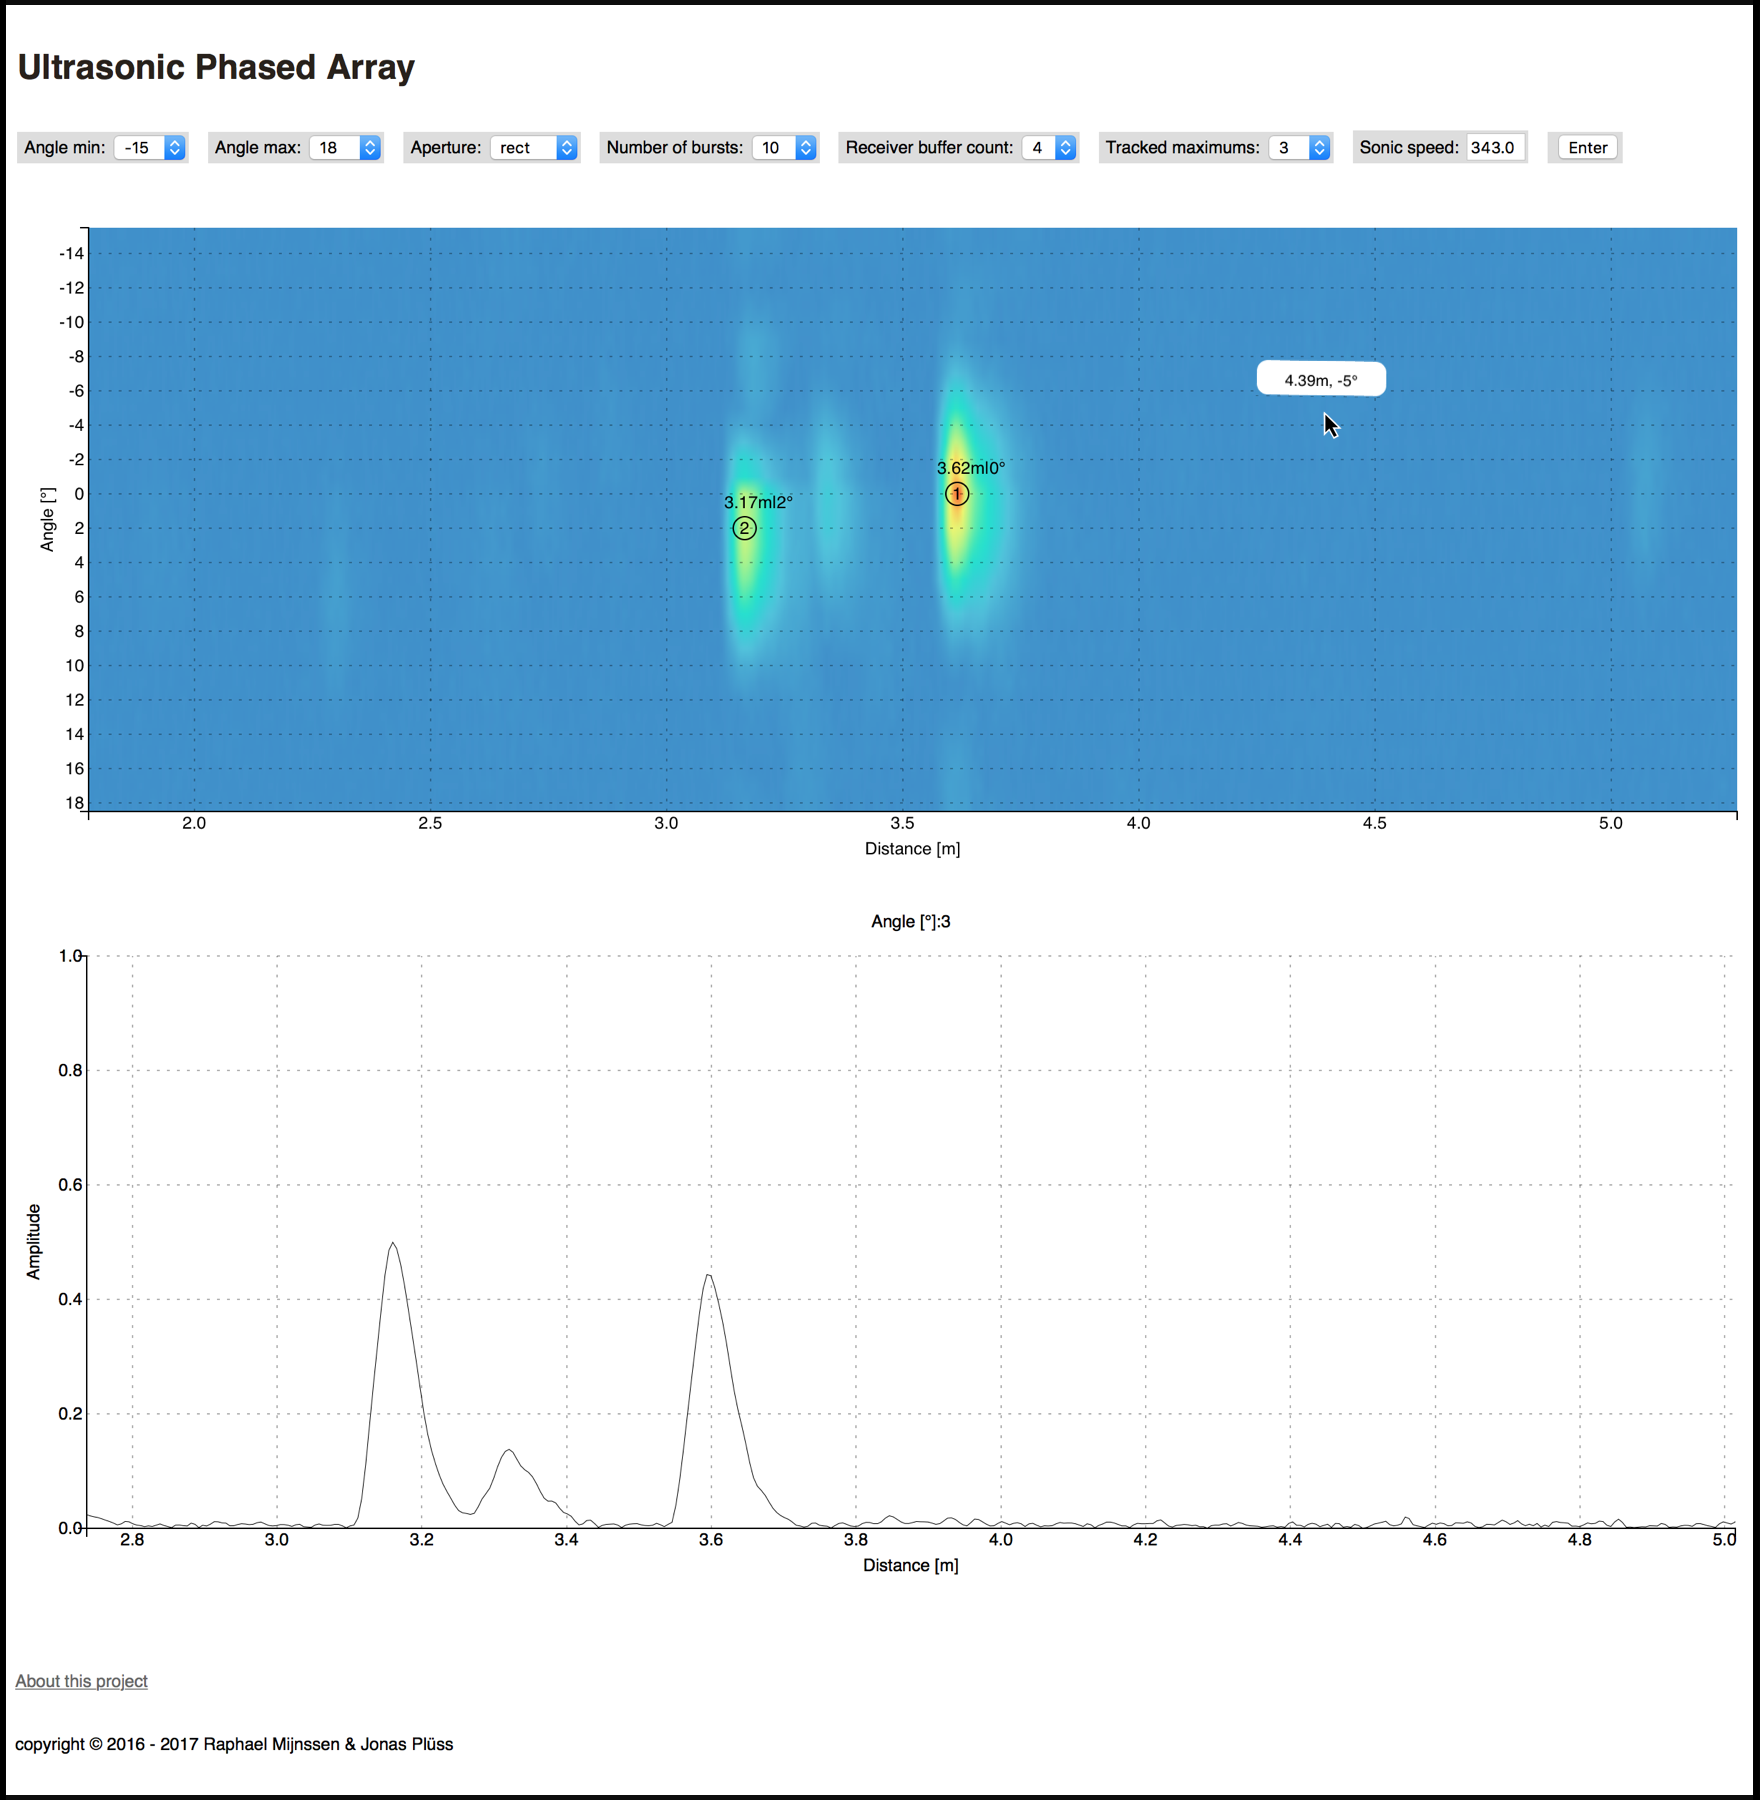
\includegraphics[width=\textwidth]{graphics/image_software_client.png}
\end{center}
\caption{Die grafische Benutzeroberfläche} % picture caption
\label{fig:image_software_client}
\end{figure}
%
%(Abb. \ref{fig:image1})
%%%%%%%%%%%%%%%%%%%%%%%%%%%%%%%%%%%%%%%%%%%%%%%%%%%%%%%%%%%%%%%%%%%%%%%%%%%%%%%%

Der Benutzer hat über die HTTP Seite \texttt{http://server\_address:5000/} Zugriff auf die grafische Benutzeroberfläche. Sobald die Seite geladen ist, laufen die Messungen mit anschliessender Darstellung der Resultate automatisch. Die Darstellungen aktualisieren sich dabei nach jedem Messvorgang. Beide Graphen sind zoom- und schiebbar. Wird der Mauszeiger über die Graphen bewegt, werden mithilfe von Tooltips Informationen zur Position im Graph eingeblendet (Winkel und Distanz im oberen Graph in Abbildung \ref{fig:image_software_client}).

Die Webseite kann grob in 3 Bereiche unterteilt werden:

\begin{itemize}
	\item Eingaben
	\item Heatmap-Graph
	\item Linienplot
\end{itemize}

 Im ersten Bereich sind die Eingabeformulare zu sehen. Der Benutzer kann dort folgende Einstellungen verändern:

\begin{itemize}
	\item Minimaler Winkel und maximaler Winkel: Der Bereich dazwischen wird ''gescannt'' (Maximal $\pm 30^{\circ}$)
	\item Aperture: Auswahl der Amplitudenbelegung (Rechteck,$\cos$, $\cos^{2}$ oder Gauss)
	\item Number of Bursts: Anzahl Sendepulse (Gerade Zahl zwischen $0$ und $80$)
	\item Receiver Buffer Count: Anzahl Daten Puffer ($1$,$2$,$4$ oder $8$ / bestimmt die Messdauer)
	\item Tracked Maxima: Anzahl Maxiums welche verfolgt/gespeichert werden ($0$ - $15$)
	\item Sonic Speed: Schallgeschwindigkeit
\end{itemize}


Im Heatmap-Graph (erster Graph in Abbildung \ref{fig:image_software_client}) ist ein ''Bild'' der Umgebung zu sehen. Die y-Achse ist der ausgewählte Winkelbereich und die x-Achse die Distanz. Farblich codiert wird die Stärke von Echos aus dem jeweiligen Winkel aufgetragen. Es handelt sich dabei um das im Kapitel \ref{sec:signalverarbeitung} beschriebene Signal. Die zeitliche Information dieses Signals (x-Achse) entspricht der zurückgelegten Distanz des Schalls.
Für jede neue Messung wird jeweils eine Zeile im Bild an der richtigen Stelle überschrieben. Die Scanrichtung verläuft vom minimalen Winkel zum maximalen Winkel. Falls das ''Maximum Tracking'' aktiviert ist, werden gefundene Maxima mit dazugehörigem Winkel und Distanz angezeigt (\ref{fig:image_software_client}). Diese sind der Grösse nach sortiert. Im obigen Bild entspricht das grosse Maximum der Decke in einem hohen Raum und das kleinere Maximum einer Runden Lampe, welche an der Decke befestigt ist.

Im Linienplot (zweiter Graph in Abbildung \ref{fig:image_software_client}) ist der Verlauf des zum aktuellen Sendewinkel zugehörigen Signals dargestellt. Der aktuelle Winkel ist oberhalb dieses Plots aufgetragen. Wird gewünscht, dass nur in einem Winkel gesendet wird, so können beide Winkeleingaben im GUI auf den selben Winkel gestellt werden. Die Amplituden-Angabe ist normiert auf einen gemessenen Maximalwert. Da es sich nicht um ein Schalldruck-Messgerät handelt, wird auf eine Referenzmessung verzichtet.

\subsubsection{HTML und CSS}\label{sec:html_und_css}
Die Webseite, welche das GUI zur Verfügung stellt, ist in HTML geschrieben. Es werden die Eingabeformulare (oben in Abbildung \ref{fig:image_software_client}) erzeugt und Javascript-Code ausgeführt, welcher die Graphen erzeugt.
Der HTML-Source-Code wird von der Flask-Applikation zur Laufzeit des Programms dynamisch erzeugt und an den Client übergeben (\ref{sec:hauptprogramm}). Beim Source-Code, der vom Flask-Server an den Client übergeben wird, handelt es sich nicht um reinen HTML-Code. Es handelt sich um ein in der \texttt{Jinja2}-Sprache geschriebenes HTML-Template, in welchem auf Variablen der Flask-Applikation zugegriffen wird.

Der CSS-Code ist im Gegensatz zum HTML-Code statisch. In den zwei Files ''style.css'' und ''style\_plot.css'' sind die Darstellungsoptionen für die Webseite und die Plots gespeichert.

Sobald die Benutzereingaben bestätigt sind, werden diese per HTTP POST-Request an den Host übertragen. Danach wird der Javascript Code ausgeführt.

\subsubsection{Javascript -- plot.js}\label{sec:javascript}
Im File ''plot.js'' sind Javascript-Funktionen deklariert. Diese erstellen die Graphen, updaten diese mit neuen Daten und stellen das SSE-Interface zum asynchronen Empfangen neuer Daten zur Verfügung. Die Plots werden mithilfe der Bibliothek \texttt{d3} erstellt. Diese Bibliothek vereinfacht den Umgang mit Vektorelementen im Browser und hilft dabei, dynamische und interaktive Plots zu erstellen.

Zusätzlich werden die Positionen der Maxima im ausgewählten Winkelbereich mit einer Javascript-Funktion berechnet. Konsequenterweise müsste dieses Maximum-Tracking auf dem Server stattfinden, mit der restlichen Signalverarbeitung. Durch eine Berechnung im Client kann jedoch der Server entlastet werden. Somit kann z.B. ein Raspberry Pi als Host eingesetzt werden.

Aus dem HTML-File werden die Javascript Funktionen folgendermassen aufgerufen:

\begin{lstlisting}[frame=single]
tracking_obj = start_maximum_tracking(numb_of_maximums);

timeseries_graph = make_timeseries_plot(''#time_series_plot'');
heatmap_graph = make_heatmap_plot(''#heatmap_plot'', maximum_tracking_obj);

sse_listener(heatmap_graph.update_plot, timeseries_graph.update_plot);
\end{lstlisting}

Die Funktion \texttt{start\_maximum\_tracking(n)} speichert Informationen zu den \texttt{n} grössten Peaks im gescannten Winkelbereich im Objekt \texttt{tracking\_obj}.
Die Aktualisierung dieser Maxima findet beim Eintreffen neuer Daten statt. Es wird dabei nur das neuste Signal untersucht. Als erstes werden Peaks gesucht und diese gespeichert. Es wird der Euklidische Abstand dieser Peaks zu den bereits gespeicherten Maxima berechnet (Distanz zu den entsprechenden Punkten im Heatmap-Graph). Schlussendlich wird anhand dieses Abstands entschieden, welche dieser neuen Peaks gespeichert werden sollen, sodass keine Maxima direkt nebeneinander liegen.

Die Funktionen zum Erzeugen der Plots erwarten als Übergabeparameter die ID des HTML-Div-Containers, in welchem der Plot gezeichnet werden soll. Der Funktion zum Erzeugen der Heatmap kann ein weiterer Übergabeparameter mitgegeben werden. Wird als zweites Element das \texttt{tracking\_obj} übergeben, so werden die darin gespeicherten Maxima im Plot dargestellt.
Als Rückgabeparameter geben die Funktionen jeweils ein Objekt zurück, über welches eine Funktion \texttt{update\_plot(new\_data)} aufgerufen werden kann. Damit können die Plots aktualisiert werden.

Der Heatmap-Plot wird aus Teilbildern zusammengesetzt, die in ein HTML5-Canvas-Element gezeichnet werden. Für jedes neue Signal wird eine Zeile im Bild ersetzt. Jedes Pixel des Bildes entspricht dabei einem Abtastwert aus einem Signal. Dieses Bild wird als unsichtbares HTML5-Canvas gespeichert. Je nach Zoom-/Schiebeeinstellung wird ein skalierter Ausschnitt davon auf ein sichtbares HTML5-Canvas-Element gezeichnet.

Die Funktion \texttt{sse\_listener(functions)} ist ein Eventlistener. Sie ruft alle ihr übergebenen Funktionen auf, sobald ein neuer Server Sent Event (siehe Kapitel \ref{sec:hauptprogramm}) eingetroffen ist. Dabei übergibt sie diesen Funktionen die neuen Daten. Ihr werden die beiden \texttt{update\_plot} Funktionen übergeben.



\clearpage
%%%%%%%%%%%%%%%%%%%%%%%%%%%%%%%%%%%%%%%%%%%%%%%%%%%%%%%%%%%%%%%%%%%%%%%%%%%%%%%%
%%%%%%%%%%%%%%%%%%%%%%%%%%%%%%%%%%%%%%%%%%%%%%%%%%%%%%%%%%%%%%%%%%%%%%%%%%%%%%%%
%%%%%%%%%%%%%%%%%%%%%%%%%%%%%%%%%%%%%%%%%%%%%%%%%%%%%%%%%%%%%%%%%%%%%%%%%%%%%%%%
\subsection{Entwicklungsumgebung}\label{sec:entwicklungsumgebung}
Im folgenden Kapitel ist beschrieben, welche Software für die Entwicklung des Projektes verwendet wird. Anhand dieser Beschreibung soll es möglich sein, eine eigene Entwicklungsumgebung aufzusetzen, in welcher das Projekt weiterentwickelt werden kann.

Als Entwicklungsbetriebssystem wird für das ganze Projekt GNU/Linux Debian in verschiedenen Versionen verwendet. Die älteste getestete Version ist Debian 8.0. Sämtliche nachfolgenden Beschreibungen beziehen sich auf die Verwendung einer vergleichbaren Installation. Grundsätzlich wurde aber während des gesamten Projektverlaufs grosser Wert darauf gelegt, plattformunabhängig zu entwickeln. Es ist auch möglich, das Projekt auf einem Microsoft Windows- oder einem Mac-System zum Laufen zu bringen. Die grösste Stolperfalle unter Windows/MacOS ist dabei eine fehlende Installation der USB-Bibliothek \texttt{libusb}.

Die folgende Grafik \ref{fig:image_software_folder_structure} zeigt die Struktur des Projektordners.
%%%%%%%%%%%%%%%%%%%%%%%%%%%%%%%%%%%%%%%%%%%%%%%%%%%%%%%%%%%%%%%%%%%%%%%%%%%%%%%%
\begin{figure}[htb]
\dirtree{%
.1 ./.
	.2 datasheets/.
		.3 external/\_module\DTcomment{Datenblätter für das externe Sendemodul}.
		.3 ultrasonic\_controller/\DTcomment{Datenblätter für die Phased Array Hardware}.
	.2 documentation/.
		.3 simulationen/\DTcomment{LTSpice und k-Wave Simulationen}.
		.3 fachbericht/\DTcomment{\LaTeX -Sourcecode des Fachberichts}.
		.3 pflichtenheft/\DTcomment{\LaTeX -Sourcecode des Pflichtenhefts}.
	.2 hardware/.
		.3 external\_module/\DTcomment{Hardware für das externe Sendemodul}.
		.3 ultrasonic\_controller\_v0.1/\DTcomment{Phased Array Hardware des Projekt 5}.
		.3 ultrasonic\_controller\_v0.2/\DTcomment{Phased Array Hardware des Projekt 6}.
	.2 software/.
		.3 firmware\_external\_module\DTcomment{Firmware für das externe Sendemodul/}.
		.3 firmware\_ultrasonic\_controller/\DTcomment{Firmware für die Phased Array Hardware}.
			.4 firmware/\DTcomment{Schutz der darüberliegenden Ordnerstruktur}.
		.3 server\_flask/\DTcomment{Flask Server Software (GUI)}.
		.3 testing\_utilities/\_and\_backup\DTcomment{Verschiedene Test- und Verifikationssoftware}.
}
\caption{Struktur des Projektordners} % picture caption
\label{fig:image_software_folder_structure}
\end{figure}
%%%%%%%%%%%%%%%%%%%%%%%%%%%%%%%%%%%%%%%%%%%%%%%%%%%%%%%%%%%%%%%%%%%%%%%%%%%%%%%%

Viele Vorgänge in dem Projektordner wurden mithilfe von Makefiles automatisiert. So können zum Beispiel im Dokumentationsordner der Fachbericht und das Pflichtenheft per \texttt{make} Befehl generiert werden, und auch die Firmware wird per Makefile kompiliert und auf dem Mikrocontroller des Arduino DUE geladen. Die Ordnerstruktur sollte soweit selbsterklärend sein, bis auf ein kleines Detail. Der Ordner \texttt{./software/firmware\_ultrasonic\_controller} enthält einen weiteren Ordner \texttt{firmware}, der den darüberliegenden Ordner vor Veränderungen durch das Makefile schützt. Dieses generiert während dem Kompiliervorgang eine Ordnerstruktur mit Binärdateien im Ordner \texttt{./software/firmware\_ultrasonic\_controller}.

\subsubsection{Hardwareentwicklung}\label{sec:hardwareentwicklung}
Das Schema und der PCB für die Hardware sind mithilfe des opensource Programms Kicad entwickelt. Dieses PCB-Design-Tool steht unter der GPL und wird unter anderem vom CERN mitentwickelt.

Kicad ist in seiner Grundinstallation mit relativ grossen Bauteilbibliotheken ausgestattet, so dass nur von wenigen Komponenten Schema und Footprint gezeichnet werden müssen. Ausserdem können damit ohne grossen Aufwand auch mehrlagige PCB's entwickelt werden, wovon in diesem Projekt mit einem vierlagigen Print Gebrauch gemacht wurde.

\subsubsection{Entwicklungsumgebung für die Firmware}\label{sec:entwicklungsumgebung_fuer_die_firmware}
Wie schon im Kapitel \ref{sec:hardware} erläutert, wird als Hardwareumgebung für den Mikrocontroller das Arduino DUE Board verwendet. Es besitzt einen 32-Bit Mikrocontroller des Typs SAM3X8E. Naheliegend wäre als Softwareumgebung dementsprechend die Arduino IDE. Darauf wird aber bewusst verzichtet, da die Arduino IDE einerseits hauptsächlich für 8-Bit Mikrocontroller entwickelt wurde und daher nicht alle Funktionalitäten des SAM3X8E unterstützt und andererseits einigen unnötigen Ballast mit sich bringt, den man nur schwer entfernen kann. Auch ein Herauslösen einzelner Module aus den Arduino Bibliotheken ist aufgrund ihrer stark verstrickten Abhängigkeiten sehr aufwändig.

Stattdessen wird das Atmel Software Framework (ASF) verwendet, welches sehr viele Treiber für den benutzten Mikrocontroller beinhaltet. Leider umfasst das ASF insgesamt mehr als $1.5 \mathrm{GB}$ an Daten, wovon nur ein Bruchteil für das Projekt überhaupt gebraucht werden. Mithilfe des Atmel Studios wurden einmalig die für das Projekt benötigten Bibliotheken aus dem ASF extrahiert und separat gespeichert, wodurch sich die Sourcecodegrösse der ASF auf $5.9 \mathrm{MB}$ reduzieren liess. Dadurch wird einerseits die Pflege des ganzen Projektcodes und andererseits auch die Fehlersuche beim Debuggen des eigenen Sourcecodes vereinfacht.

Zum Kompilieren des Sourcecodes greift das Atmel Software Framework im Hintergrund auf den gcc-arm-none-eabi zurück, welcher auf der GNU Compiler Collection (GCC) aufbaut. Darin sind alle Werkzeuge enthalten, welche zum Kompilieren und Linken von C-Code für den SAM3X8E verwendet werden. Um das kompilierte Programm auf den Mikrocontroller zu laden, wird das Programm ''Bossac'' (bossa-cli) verwendet. Der ganze Kompilier- und Ladevorgang wird über ein Makefile aus dem Atmel Software Framework gesteuert, welches für unsere Zwecke angepasst wurde.

Nachfolgend befindet sich eine kurze Auflistung aller Programme, welche für die Entwicklung der Firmware benötigt werden:

\begin{itemize}
	\item gnu make			v4.0
	\item gcc-arm-none-eabi		v4.8.4
	\item bossac (bossa-cli)	v1.3a
	\item Doxygen (optional zum Dokumentieren des Sourcecodes)
\end{itemize}

Die Versionsnummern geben jeweils die älteste erfolgreich getestete Version der einzelnen Programme an. Es ist durchaus möglich, dass auch noch ältere Versionen funktionieren, dies wurde aber nicht verifiziert.


\clearpage
\subsubsection{Installation auf dem Desktop Betriebssystem}\label{sec:installation_auf_dem_desktop_betriebssystem}
Um die Hardware ansteuern zu können, braucht es ein Desktop Betriebssystem, auf welchem Server und Client ausgeführt werden. Diese sind in Python, HTML, CSS und Javascript geschrieben. Auf dem System, an welchem die Hardware per USB angeschlossen ist und auf dem der Flask Server laufen soll, muss eine funktionierende Pythonumgebung mit folgenden Paketen installiert werden:

\begin{itemize}
	\item numpy	v1.8.2
	\item scipy	v0.14.0
	\item pyusb	v1.0.0
	\item flask	v0.10.1
	\item wtforms	v2.0.1
	\item gevent	v1.0.1
\end{itemize}

Die Versionen beziehen sich auch hier auf die niedrigste getestete Version. Ausser dem Paket ''pyusb'' können auf dem verwendeten Debian 8 System alle Pakete über die offiziellen Quellen installiert werden. Bei ''pyusb'' muss die Installation von Hand ausgeführt werden, da sich in den offiziellen Quellen eine zu alte Version befindet. Am einfachsten installiert man sich dazu das Programm ''pip'' (python-pip) und installiert das Paket per Befehl \texttt{pip install -{}-upgrade pyusb} auf dem System. Auf einer Debian 9 Installation tritt dieses Problem nicht mehr auf.

Um auf den Server zuzugreifen, verwendet man am besten den Browser ''Firefox'', da der Java\-script Code hauptsächlich auf diesem Browser entwickelt und getestet wurde. Im Browser muss Javascript eingeschaltet werden.


\subsubsection{Bedienungsanleitung}\label{sec:bedienungsanleitung}
Im Folgenden wird beschrieben, wie das Ultraschall Phased Array-System in Betrieb genommen wird. Es wird empfohlen dafür ein Linux-Betriebssystem zu verwenden, der Server wurde jedoch auch unter Windows und Mac OS X erfolgreich getestet.

Ist ein Arduino DUE mit der aktuellen Firmware vorhanden, so muss nur noch der Server (Host) in Betrieb genommen, und mit einem Webbrowser darauf zugegriffen werden. Dafür muss das Desktop-Betriebssystem nach der Beschreibung im Kapitel \ref{sec:installation_auf_dem_desktop_betriebssystem} eingerichtet sein.

Der Arduino DUE muss über den ''native USB'' Port mit dem System verbunden sein. Danach kann der Server mit folgendem Befehl gestartet werden (alle relativen Pfadangaben beziehen sich auf den Projektordner):

\texttt{python ./software/server\_flask/server\_flask.py}

In der Shell wird nach jeder Messung mit der Ausgabe: \texttt{ServerFlask: callback function} signalisiert, dass neue Daten vorhanden sind.

Über einen Firefox-Webbrowser wird das User-Interface mit folgender Adresse aufgerufen:

\texttt{http://localhost:5000/}

Wird von einem anderen System aus über ein Netzwerk auf den Server zugegriffen, so muss \texttt{localhost} mit der Adresse des Servers ersetzt werden.
Sobald die Daten vom Webbrowser abgeholt werden, wird dies in der Shell mit der Ausgabe: \texttt{ServerFlask: event
} bestätigt.

Falls sich die Firmware nicht auf dem Arduino DUE befindet, muss die im Kapitel \ref{sec:entwicklungsumgebung_fuer_die_firmware} beschriebene Entwicklungsumgebung eingerichtet werden. Der Arduino DUE muss anschliessend zurückgesetzt werden (Reset-Button). Um die Firmware zu installieren, wechselt man seinen Arbeitsordner zu: \texttt{./software/firmware\_ultrasonic\_controller/firmware/}. Mit folgendem Befehl wird die Firmware auf dem Arduino DUE installiert:

\texttt{make install}

Dafür sind Rootrechte nötig.

\subsubsection{Lizenzen}
Die in diesem Projekt entwickelte Soft- und Hardware werden unter den Bedingungen der GNU GPL v3 (GNU General Public License) freigegeben. Das Atmel Software Framework, aus dem der USB Stack und weitere Treiber für ADC, Timer, PWM, usw. verwendet werden, steht unter einer Lizenz von Atmel, welche im Anhang \ref{sec:appendix_lizenzen} zu finden ist.
